

\chapter{含参积分}

\section{含参正常积分}

\subsection{含参正常积分基本概念与定理}

\begin{definition}[含参正常积分]
  $f(x,t)$是定义于$G = \{\alpha(t) \leq x \leq \beta(t), a \leq t \leq b\}$区域的二元函数,
  当对$x$积分时,该积分为$t$的函数:
  \begin{equation*}
    F(t) = \int_{\alpha(t)}^{\beta(t)} f(x,t) \mathrm{d} x, t \in [a,b]
  \end{equation*}
\end{definition}

\begin{theorem}[规则区域含参正常积分性质]
  若$f(x,t)$在$[a,b] \times [c,d]$连续,则
  \begin{itemize}
  \item 连续性:含参积分连续,
    即对$\forall t_0 \in [c,d]$有$\lim \limits _{t \rightarrow t_0} \int_a^b f(x,t)\mathrm{d} x = \int_a^b f(x,t_0)\mathrm{d} x$
  \item 积分交换:$\int_c^d \mathrm{d} t \int_a^b f(x,t)\mathrm{d} x = \int_a^b \mathrm{d} x \int_c^d f(x,t)\mathrm{d} x$
  \item 可导:若$f_t(x,t)$在$[a,b] \times [c,d]$也连续,则
    $ \frac{\mathrm{d} }{\mathrm{d} t}\left(  \int_a^b f(x,t)\mathrm{d}x\right) = \int_a^b f_t(x,t)\mathrm{d}x  $
  \end{itemize}
\end{theorem}

\begin{theorem}[不规则区域的连续与可微性]
  若$f(x,t)$在$[\alpha(t),\beta(t)] \times [c,d]$连续,$\alpha(t),\beta(t)$在$[c,d]$上连续,
  则
  \begin{itemize}
  \item 连续性:$\varphi(t) = \int_{\alpha(t)}^{\beta(t)} f(x,t)\mathrm{d} x$在$[c,d]$上连续,
    即
    \begin{equation*}
      \forall t_0 \in [c,d], \lim \limits _{t \rightarrow t_0}\varphi(t) = \int_{\alpha(t_0)}^{\beta(t_0)} f(x,t_0)\mathrm{d}x
    \end{equation*}
  \item 可微性:若$f_t(x,t)$在$[a,b] \times [c,d]$上连续,
    $\alpha(t),\beta(t)$在$[c,d]$上可导,则(将被积分变量用上下限代替)
    \begin{equation*}
      \varphi^{\prime}(t) = f(\beta(t),t)\beta^{\prime}(t) - f(\alpha(t),t)\alpha^{\prime}(t) + \int_{\alpha(t)}^{\beta(t)}f_t(x,t)\mathrm{d} x
    \end{equation*}
  \end{itemize}
\end{theorem}

~

\begin{exercise}[含参积分求导]
  (1)重点:已知$f(x) \in C[a,b]$,
  $F(y) = \int_a^b f(x)|y - x| \mathrm{d} x, y \in [a,b]$,
  计算$F^{\prime\prime}(y)$
\end{exercise}

\begin{solution}
  (1)首先得改写为不规则区域积分:$F(y) = \int_a^y f(x)(y - x)\mathrm{d} x + \int_y^b f(x)(x - y)\mathrm{d} x$,
  因此
  \begin{equation*}
    F^{\prime}(y) = f(y)(y-y)\cdot 1 + \int_a^y f(x)\mathrm{d} x - f(y)(y-y) - \int_y^b f(x)\mathrm{d} x = \int_a^y f(x)\mathrm{d} x - \int_y^b f(x)\mathrm{d} x
  \end{equation*}
  进而得到$F^{\prime\prime}(y) = f(y) + f(y) = 2f(y)$
\end{solution}

~


\begin{exercise}[含参积分求导的应用]
  (1)计算极限$\lim \limits _{x \rightarrow 0} \frac{\int_0^{x^2} \sqrt{1 + t^2}\mathrm{d} t}{e^x \sin x - \sin x}$
\end{exercise}

\begin{solution}
  (1)方法一:使用含参积分求导,
  分母等价于$(1+x)x - x = x^2$,
  使用洛必达法则得到(注意分子是含参积分求导):
  \begin{equation*}
    \lim \limits _{x \rightarrow 0}\frac{2x \sqrt{1 + x^4}}{2x} = \lim \limits _{x \rightarrow 0} \sqrt{1 + x^4} = 1
  \end{equation*}

  方法二:Taylor展开+直接积分:
  分母等价于$x^2$,
  分子用$\sqrt{1 + t^2} = 1 + \frac{t^2}{2} + o(t^2)$得到:
  \begin{equation*}
    I = \lim \limits _{x \rightarrow 0} \frac{\int_0^{x^2} 1 + \frac{t^2}{2} + o(t^2) \mathrm{d} t}{x^2} = \lim \limits _{x \rightarrow 0} \frac{x^2 + \frac{x^6}{6} + o(x^{^6})}{x^2} = 1
  \end{equation*}
\end{solution}

\subsection{常用含参正常积分的计算}

\begin{lemma}
  $|a| < 1$时,$\int \frac{\mathrm{d} x }{1 + a \cos x} = \frac{2}{\sqrt{1 - a^2}} \arctan \left( \sqrt{\frac{1-a}{1+a}} \tan \frac{x}{2} \right) + C$,
  特别地,$\int_0^{\pi} \frac{\mathrm{d} x}{1 + a \cos x} = \frac{\pi}{\sqrt{1 - x^2}}$
\end{lemma}

\begin{proof}
  使用万能公式,在前面三角函数不定积分中涉及过。
\end{proof}

~

\begin{exercise}[积分:涉及$\frac{x^b - x^a}{\ln x}$型]
  (1)计算$\int_0^1 \frac{x^b - x^a}{\ln x}\mathrm{d} x, 0 < a < b$

  (2)计算$\int_0^1 \sin \left( \ln \frac{1}{x} \right) \frac{x^b - x^a}{\ln x}\mathrm{d}x$

  (3)计算$F(a) = \int_0^{\frac{\pi}{2}} \ln \frac{1 + a \cos x}{1 - a \cos x} \cdot \frac{1}{\cos x}\mathrm{d} x$,这里$a \in (-1,1)$
\end{exercise}

\begin{solution}
  (1)由于$\int_a^b x^y\mathrm{d} y = \frac{x^y}{\ln x} \bigg|_a^b = \frac{x^b - x^a}{\ln x}$,
  因此根据交换积分顺序得到
  \begin{equation*}
    \int_0^1 \frac{x^b - x^a}{\ln x}\mathrm{d}t = \int_0^1 \mathrm{d} x \int_a^b x^y\mathrm{d} y = \int_a^b \mathrm{d} y \int_0^1 x^y \mathrm{d} x = \ln \frac{1 + b}{1+a}
  \end{equation*}

  (2)由于$\int_a^b x^y \mathrm{d} y = \frac{x^b - x^a}{\ln x}$,
  而$x = 0$为瑕点,考虑$\lim \limits _{x \rightarrow 0} \sin \left( \ln \frac{1}{x} \right) x^y = 0$,
  因此可视为连续。
  从而
  \begin{equation*}
    \int_0^1 \sin \left( \ln \frac{1}{x} \right) \frac{x^b - x^a}{\ln x}\mathrm{d} x = \int_a^b \mathrm{d} y \int_0^1 \sin \left( \ln \frac{1}{x} \right)x^y \mathrm{d} x
  \end{equation*}
  令$u = \ln \frac{1}{x}$即可转化为$\int_a^b \mathrm{d} y \int_0^{+\infty} \sin u e^{-(y+1)u}\mathrm{d} u$,
  结果为$\arctan(b + 1) - \arctan (a + 1)$

  (3)注意到
  \begin{equation*}
    \ln \frac{1 + a \cos x}{1 - a \cos x} \cdot \frac{1}{\cos x}\mathrm{d} x = \frac{\ln(1 + a \cos x) - \ln(1 - a \cos x)}{\cos x} = \int_{-a}^a \frac{\mathrm{d} y}{1 + y \cos x}
  \end{equation*}
  而$\frac{y}{1+y\cos x}$连续,因此
  \begin{align*}
    F(a) = \int_{-a}^a \mathrm{d} y \int_0^{\frac{\pi}{2}} \frac{1}{1 + y \cos x}\mathrm{d} x
  \end{align*}
  最终积分结果为$\pi \arcsin a$
\end{solution}

~






\section{含参反常积分与一致收敛}

\subsection{基本概念}

\begin{definition}[含参反常积分]
  $f(x,t)$在$[c,+\infty) \times I$上有定义,
  对$\forall t \in I$,
  反常积分$\int^{+\infty}_cf(x,t)\mathrm{d}x$收敛,
  则记$\Phi(t) = \int^{+\infty}_c f(x,t)\mathrm{d}x$,称其为含参反常积分。
\end{definition}

\begin{definition}[含参反常积分一致收敛]
  若对$\forall \epsilon, \exists N > c, \forall M > N, \forall t \in I$有
  $|\int^{+\infty}_M f(x,t) \mathrm{d}x | < \epsilon$,
  则称$\int^{+\infty}_c f(x,t)\mathrm{d}x$一致收敛于$\Phi(t)$
\end{definition}

\begin{theorem}[一致收敛基本充要条件]
  含参反常积分一致收敛有以下两个基本充要条件:
  \begin{itemize}
  \item Cauchy收敛准则:$\forall \epsilon, \exists M > c, \forall A_1,A_2 > M, \forall t \in I$满足$|\int_{A_1}^{A_2} f(x,t)\mathrm{d}x| < \epsilon$
  \item 上确界判别法:$\lim \limits _{A \rightarrow +\infty} \sup \limits _{t \in I}|\int_A^{+\infty}f(x,t)\mathrm{d}x| = 0$。
  \end{itemize}
\end{theorem}

\begin{note}
  证明不一致收敛一般用上确界判别法,具体见下面的例子
\end{note}

~

\begin{exercise}[重要例子:确界判别]
  证明$\int_0^{+\infty} \frac{\sin xy}{y}\mathrm{d} y$在$[\delta, +\infty)$上一致收敛,
  但在$(0,+\infty)$上不一致收敛
\end{exercise}

\begin{proof}
  (1)一致收敛:做变量替换$u = xy$得到$\int_A^{+\infty} \frac{\sin xy}{y}\mathrm{d} y = \int_{Ax}^{+\infty} \frac{\sin u}{u}\mathrm{d} u$,
  根据反常积分Dirichlet判别法可知$\int_0^{+\infty} \frac{\sin u}{u}\mathrm{d}u $收敛,
  因此$\forall \epsilon, \exists M, \forall A^{\prime} > M$时,有
  \begin{equation*}
    \left| \int_{A^{\prime}}^{+\infty} \frac{ \sin u}{u}\mathrm{d} u \right| < \epsilon
  \end{equation*}
  对题中的$\delta$,取$A > \frac{M}{\delta}$,
  当$x \geq \delta$时有
  \begin{equation*}
    \left| \int_A^{+\infty} \frac{\sin xy}{y}\mathrm{d}y \right|< \epsilon
  \end{equation*}
  因此根据确界判别法可知一致收敛。

  (2)不一致收敛:
  因为
  \begin{equation*}
    \sup \limits_{x \in (0,+\infty)} \left| \int_A^{+\infty} \frac{\sin xy}{y}\mathrm{d} y \right| = \sup \limits_{x \in (0,+\infty)} \left| \int_{Ax}^{+\infty } \frac{\sin u}{u}\mathrm{d} u \right| \geq \left| \int_0^{+\infty} \frac{\sin u}{u}\mathrm{d} u \right| = \frac{\pi}{2}
  \end{equation*}
  当$A \rightarrow +\infty$时,极限不趋于$0$,因此根据上确界准则可知不一致收敛。
\end{proof}

\begin{note}
  本题在$[\delta,+\infty)$上也可以用Dirichlet判别法,
  在$(0,+\infty)$无法用的原因在于$\int_0^N \sin xy \mathrm{d} y = \frac{\cos xy}{x} \bigg|_0^N$对$x \in [0,+\infty)$不一致有界。
\end{note}

~

\begin{exercise}[不一致收敛例子]
  (1)讨论$\varphi(x) = \int _0^{+\infty}x e^{-xy}\mathrm{d}y$在$(0,+\infty)$上的一致收敛性
\end{exercise}

\begin{solution}
  (1)$\varphi(x) = \int_0^{+\infty}e^{-xy}d(xy) = e^{-xy}|_{+\infty}^0 = 1$,
  但是其不一致收敛,原因是$\sup \limits_{x \in (0,+\infty)}|\int_M^{+\infty}xe^{-xy}\mathrm{d}y| 
  = \sup \limits_{x \in (0,+\infty)} e^{-Mx} = 
  1$不趋于$0$。
  (如果$x \in (a,+\infty), a > 0$则一致收敛)
\end{solution}

~

\begin{theorem}[M判别法]
  若$g(x)$满足$|f(x,t)| \leq g(x), x \in [c,+\infty), t \in I$,
  且$\int_c^{+\infty}g(x)\mathrm{d}x$收敛,则
  $\int_c^{+\infty}f(x,t)\mathrm{d}x$在$I$上一致收敛。
\end{theorem}

\begin{theorem}[比较判别法]
  $f(x,t)$在$[c,+\infty) \times I$上连续,$|f(x,t)| \leq F(x,t)$,
  若$\int_c^{+\infty}F(x,t)\mathrm{d}x$在$I$上一致收敛,
  则$\int_c^{+\infty}f(x,t)\mathrm{d}x$在$I$上绝对一致收敛
\end{theorem}

\begin{proof}
  根据Cauchy收敛准则可知$\forall \epsilon, \exists M, \forall A_1,A_2 > M, \forall t, |\int_{A_1}^{A_2}F(x,t)\mathrm{d}x| < \epsilon$,
  因此推出$\int_{A_1}^{A_2}|f(x,t)| \mathrm{d}x < \epsilon$。
\end{proof}

~

\begin{exercise}[M判别法]
  (1)证明$\int_0^{+\infty} \frac{\cos xy}{1 + x^2}\mathrm{d} x$在$(-\infty,+\infty)$上一致收敛
  
  (2)证明$\int_0^{+\infty}e^{-x^2y}\mathrm{d}y$在$x \in [a,b]$一致收敛
\end{exercise}

\begin{proof}
  (1)对任意$y$有$\left| \frac{\cos xy}{1 + x^2} \right| \leq \frac{1}{1+x^2}$,
  而$\int_0^{+\infty} \frac{\mathrm{d} x}{1 + x^2}$收敛,因此由$M$判别法可知一致收敛。
  
  (2)由于$e^{-x^2y} \leq e^{-a^2y}$,且根据比较原则$\int_0^{+\infty}e^{-a^2y}\mathrm{d}y$收敛
\end{proof}

\begin{note}
  即使含参反常积分是常数,也不代表其一致收敛。
\end{note}

\subsection{Dirichlet与Abel判别法}

\begin{theorem}[Dirichlet与Abel判别法]
  对于$\int_c^{+\infty}f(x,t)g(x,t)\mathrm{d}x$,满足下面的条件则一致收敛
  \begin{itemize}
  \item Dirichlet判别法:(1)$\forall N > c, \int_c^N f(x,t)\mathrm{d}x$关于$t$一致有界(2)固定$t \in I$,$g(x,t)$关于$x$单调,且$x \rightarrow \infty$时关于$t$一致收敛(即与$t$的选取无关)到$0$
  \item Abel判别法:(1)$\int_c^{+\infty} f(x,t)\mathrm{d}x$在$I$上一致收敛(2)固定$t \in I$,$g(x,t)$关于$x$单调,$g(x,t)$关于$t \in I$一致有界
  \end{itemize}
\end{theorem}

\begin{note}
  注意这里单调都是关于$x$的,一致都是关于$t$的。
\end{note}

~

\begin{exercise}[Dirichlet判别法]
  (1)证明$\int_1^{+\infty}\frac{\sin x}{1 + xe^y} \mathrm{d}x$在$[0,+\infty)$一致收敛

  (2)证明$\int_1^{+\infty} \frac{y \sin xy}{1 + y^2}\mathrm{d} y$在$(0,+\infty)$上内闭一致收敛
\end{exercise}

\begin{proof}
  (1)
  $\left|\int_1^N\sin x \mathrm{d}x\right|$关于$y$一致有界。
  $\frac{1}{1 + xe^y}$,一旦固定$y$,肯定关于$x$单调。
  由于$0 < \frac{1}{1 + xe^y} \leq \frac{1}{1 + x} \rightarrow 0$,
  因此一致收敛到$0$。
  由Dirichlet判别法可知。

  (2)对于$[a,b] \subset (0,+\infty)$,对$\forall x \in [a,b]$,有
  \begin{equation*}
    \left| \int_1^N \sin xy \mathrm{d} y \right| = \left| - \frac{\cos xy}{x} \right|^N_1 \leq \frac{2}{a}
  \end{equation*}
  而$\left| \frac{y}{1 + y^2} \right| \leq \frac{1}{2}$一致有界,且
  \begin{equation*}
    \left( \frac{y}{1+y^2} \right)^{\prime} = \frac{1-y^2}{(1+y^2)^2} \leq 0
  \end{equation*}
  因此$\frac{y}{1+y^2}$单调减,$y \rightarrow +\infty$时,$\frac{y}{1+y^2} \rightarrow 0$,
  根据Dirichlet判别法可知
\end{proof}

~

\begin{exercise}[Abel判别法]
  (1)证明$\int_0^{+\infty}e^{-xy} \frac{\sin x}{x} \mathrm{d}x$在$[0,+\infty)$上一致收敛

  (2)$\varphi(y) = \int_0^{+\infty} \frac{\sin x^2}{1 + x^y}\mathrm{d}x$在$y \in [0,+\infty)$一致收敛
\end{exercise}

\begin{proof}
  (1)$\int_0^{+\infty} \frac{\sin x}{x} \mathrm{d}x$关于$y$一致收敛。
  $e^{-xy}$关于$x$单调,且$0 < e^{-xy} \leq 1$一致有界,由Abel判别法可知

  (2)用Abel
\end{proof}

\section{含参反常积分的性质}

\subsection{含参反常积分的极限与连续性}


\begin{theorem}[连续性]
  设$f(x,t)$在$I \times [c,+\infty)$上连续,若$\Phi(t) = \int_c^{+\infty} f(x,t)\mathrm{d} x$
  在$I$上一致收敛,则$\Phi(t)$在$I$上连续,即
  \begin{equation*}
    \lim \limits _{t \rightarrow t_0} \int_c^{+\infty} f(x,t)\mathrm{d}x = \int_c^{+\infty} f(x,t_0)\mathrm{d} x
  \end{equation*}
\end{theorem}

\subsection{含参反常积分的可微性与可积性}

\begin{theorem}[可微性]
  若$f(x,t)$与$f_t(x,t)$在$[c,+\infty) \times I$上连续,
  $\Phi(t) = \int_c^{+\infty} f(x,t)\mathrm{d} x$在$I$上收敛,
  $\int_c^{+\infty} f_t(x,t)\mathrm{d} x$在$I$上一致收敛,则
  \begin{equation*}
    \frac{\mathrm{d} }{\mathrm{d} t} \int_c^{+\infty}f(x,t)\mathrm{d} x = \int_c^{+\infty} \frac{\mathrm{d}}{\mathrm{d} t}f(x,t)\mathrm{d} x
  \end{equation*}
\end{theorem}

\begin{proof}
  取任意单增趋于$+\infty$的序列$A_n$,
  令$u_n(t) = \int_{A_n}^{A_{n+1}} f_t(x,t)\mathrm{d} x$,
  转化为函数列的逐项求导问题。
\end{proof}

\begin{theorem}[可积性]
  $f(x,t)$在$[c,+\infty) \times [a,b]$上连续,
  $\Phi(t) = \int_c^{+\infty} f(x,t)\mathrm{d} x$在$[a,b]$上一致收敛,
  则
  \begin{equation*}
    \int_a^b \mathrm{d} t \int_c^{+\infty} f(x,t)\mathrm{d} x = \int_c^{+\infty} \mathrm{d} x \int_a^b f(x,t)\mathrm{d} t
  \end{equation*}
\end{theorem}

\begin{theorem}[常用的积分公式]
  设$p > 0$,则含参积分$\int_0^{+\infty} e^{-px} \frac{\sin bx - \sin ax}{x} \mathrm{d} x = \arctan \frac{b}{p} - \arctan \frac{a}{p}$
\end{theorem}

\begin{proof}
  首先$\frac{\sin bx - \sin ax}{x} = \int_a^b \cos xy \mathrm{d} y$,
  因此
  \begin{equation*}
    I = \int_0^{+\infty} \mathrm{d} x \int _a^b e^{-px}\cos xy \mathrm{d} y
  \end{equation*}
  由于$|e^{-px}\cos xy| \leq e^{-px}$,显然$\int_0^{+\infty} e^{-px}\mathrm{d} x$绝对收敛,
  因此$\int_0^{+\infty}e^{-px}\cos xy\mathrm{d}x, y \in [a,b]$一致收敛,交换积分顺序得到
  \begin{align*}
    I = \int_a^b \mathrm{d} y \int_0^{+\infty} e^{-px} \cos xy \mathrm{d} x
  \end{align*}
  根据表格法得到:
  \begin{equation*}
    \int_0^{+\infty} e^{-px}\cos xy \mathrm{d} x = - \frac{1}{p} e^{-px}\cos xy   \bigg|^{+\infty}_0 + \frac{y}{p^2} e^{-px} \sin xy   \bigg|_0^{+\infty} - \int_0^{+\infty} \frac{y^2}{p^2} e^{-px} \cos xy\mathrm{d} x 
  \end{equation*}
  因此得到$\frac{y^2 + p^2}{p^2} \int _0^{+\infty} \cos xy\mathrm{d} y = \frac{1}{p}$
  \begin{equation*}
    I = \int_a^b \frac{p}{p^2 + y^2}\mathrm{d} y = \arctan \frac{b}{p} - \arctan \frac{a}{p}
  \end{equation*}
\end{proof}


\begin{theorem}[Dirichlet积分]
  积分$\int _0^{+\infty} \frac{\sin x}{x} \mathrm{d} x = \frac{\pi}{2}$,
  进一步地,$\int_0^{+\infty} \frac{\sin ax}{x}\mathrm{d} x = \frac{\pi}{2} \text{sgn}(a)$
\end{theorem}

\begin{theorem}[正态积分公式]
  $\int_0^{+\infty} e^{-x^2}\mathrm{d} x = \frac{\sqrt{\pi}}{2}$
\end{theorem}

~

\begin{exercise}[相关练习]
  (1)$\int_0^{+\infty} \frac{e^{-a^2x^2} - e^{-b^2x^2} }{x^e}\mathrm{d} x$
\end{exercise}



\subsection{含参反常积分与函数项级数的关系}

\begin{theorem}[一致收敛级数表示法(ZJU考研考过)]
  $\int^{+\infty}_cf(x,y)\mathrm{d}y$在$I$上一致收敛的充要条件为对任一趋于无穷的递增数列$A_n$(其中$A_1 = c$),
  $\sum\limits_{n = 1}^{\infty}\int^{A_{n+1}}_{A_n}f(x,y)\mathrm{d}y$作为函数项级数$\sum\limits_{n = 1}^{\infty}u_n(x)$在$I$上一致收敛
\end{theorem}

\begin{proof}
  (1)左推右:由于一致收敛,
  因此$\forall \epsilon, \exists M > c$使得$A^{\prime\prime} > A^{\prime} > M$时,$\forall x$有
  $|\int^{A^{\prime\prime}}_{A^{\prime}} f(x,y)\mathrm{d}y| < \epsilon$,
  由于$A_n$趋于无穷,$\exists N, \forall m>n>N$有$A_m > A_n >M$,
  对$\forall x \in I$有$|u_n(x) + \cdots + u_m(x)| = |\int_{A_n}^{A_{m+1}}f(x,y)\mathrm{d}y| < \epsilon$,即右侧级数一致收敛

  (2)右推左:反设含参积分不一致收敛,$\exists \epsilon_0, \forall M > c, \exists A^{\prime\prime} > A^{\prime} > M, x^{\prime} \in I$使得
  \begin{equation*}
    \left|\int^{A^{\prime\prime}}_{A^{\prime}}f(x^{\prime},y)\mathrm{d}y\right| \geq \epsilon_0
  \end{equation*}
  先取$M_1 = \max \{1, c\}$,则$\exists A_2, A_1$满足$A_2 > A_1 > M_1$,以及$x_1 \in I$使得
  \begin{equation*}
    \left| \int_{A_1}^{A_2}f(x_1,y)\mathrm{d} y \right| \geq \epsilon_0
  \end{equation*}
  同理取$M_n = \max \{n, A_{2n - 2}\}$,有$A_{2n} > A_{2n - 1} > M_n, x_n \in I$使得
  \begin{equation*}
    \left|\int^{A_{2n}}_{A_{2n-1}}f(x_n,y)\mathrm{d}y\right| \geq \epsilon_0
  \end{equation*}
  此时$\exists \epsilon_0, \forall N, \exists n > N, \exists x_n \in I$使得
  $|u_{2n}(x_n)| = |\int^{A_{2n+1}}_{A_{2n}} f(x_n,y)\mathrm{d}y| \geq \epsilon_0$,这与函数项级数一致收敛条件矛盾(因为一致收敛要求所有$x$都趋于$0$)。
\end{proof}













\newpage


\chapter{多重积分}


\section{二重积分}

\subsection{二重积分的概念与计算}

\begin{definition}[二重积分]
  $D \subset \mathbb{R}^2$是有界集,
  对$D$做分割$T = \{\sigma_1,\cdots,\sigma_n\}$,
  则二重积分定义为
  \begin{equation*}
    \iint _D f(x,y) \mathrm{d}x\mathrm{d}y = \lim \limits _{||T|| \rightarrow 0}\sum\limits_{i = 1}^n f(\xi_i,\eta_i) s(\sigma_i) 
  \end{equation*}
\end{definition}

\begin{theorem}[二重积分与累次积分]
  对于$D = [a,b] \times [c,d]$或者$D = [a,b] \times [f_1(x),f_2(x)]$,
  方形边界二重积分可随意转换为累次积分,函数边界先积分函数边界
  \begin{equation*}
    \iint _D f(x,y) \mathrm{d}x \mathrm{d}y = \int ^b_a \mathrm{d}x \int^d_c f(x,y)\mathrm{d}y , \quad \iint_D f(x,y) \mathrm{d}x\mathrm{d}y = \int ^b_a \mathrm{d}x \int^{f_2(x)}_{f_1(x)}f(x,y)\mathrm{d}y
  \end{equation*}
\end{theorem}

\begin{note}
  二重积分的直接计算要特别关注其区域的对称性。
  而累次积分的顺序一般看函数,那边容易积就先积(也得靠经验觉得哪个好积)。
\end{note}

~

\begin{exercise}[对称性计算]
  (1)计算$\iint_D x^2y \mathrm{d}x\mathrm{d}y$,其中$D: |x| + |y| \leq 1$
\end{exercise}

\begin{solution}
  (1)由于$D$关于$x$轴对称,且$f(x,y) = x^2y$关于$y$为奇函数,
  因此$\iint_D x^2 y\mathrm{d}x \mathrm{d}y = 0$
\end{solution}

~

\begin{exercise}[转换为累次积分]
  (1)计算$I = \iint _D e^{-y^2}\mathrm{d}x\mathrm{d}y$,其中$D$是$y = x$与$y = x^{\frac{1}{3}}$围成的区域

  (2)计算$I = \iint _D \frac{\sin x}{x} \mathrm{d}x\mathrm{d}y$,其中$D$是$y = x$与$y = x^2$围成的区域

  (3)圆周边界:计算$I = \iint _D \frac{\mathrm{d}x\mathrm{d}y}{\sqrt{2a - x}}$,其中$D$为$x = 0, y = 0$与$(x - a)^2 + (y - a)^2 = a^2$所围成的区域
\end{exercise}

\begin{solution}
  (1)注意要先积$x$,因为$e^{-y^2}$先积$x$比较方便,答案为$\frac{1}{e}$

  (2)注意要先积$y$,因为显然$\frac{\sin x}{x}$不好积,答案为$1 - \sin 1$

  (3)这里$\int \frac{1}{\sqrt{2a - x}}\mathrm{d}x$看成$\int (2a - x)^{-\frac{1}{2}}\mathrm{d}x$就是个幂函数,不要被吓到。
  先积$y$,得到
  \begin{equation*}
    I = \int_0^a \mathrm{d}x \int_0^{a - \sqrt{2ax - x^2}} \frac{1}{\sqrt{2a - x}}\mathrm{d}y = \int _0^a \frac{a - \sqrt{2ax - x^2}}{\sqrt{2a - x}} \mathrm{d} x= (2 \sqrt{2} - \frac{8}{3})a^{\frac{3}{2}}
  \end{equation*}
\end{solution}

~

\begin{exercise}[几个进阶题]
  (1)计算$I = \iint_D |xy - \frac{1}{4}| \mathrm{d}x\mathrm{d}y$,其中$D: [0,1]\times [0,1]$(补区域技巧)

  (2)计算$I = \iint_D \sqrt{|y - x^2|}\mathrm{d}x\mathrm{d}y$,其中$D: -1 \leq x \leq 1, 0 \leq y \leq 2$(对称性)
\end{exercise}

\begin{solution}
  (1)要画出$xy = \frac{1}{4}$线,分成上下两个部分,记上面的为$D_1$,下面的是$D_2$,
  但是$D_2$过于不规则,可以为$D_2$补上$D_1$的部分,这样算起来就方便不少。
  即$I = \iint _{D_1}(xy - \frac{1}{4})\mathrm{d}x\mathrm{d}y - \iint _{D_2} (xy - \frac{1}{4})\mathrm{d}x\mathrm{d}y = 2\iint _{D_1} (xy - \frac{1}{4})\mathrm{d}x\mathrm{d}y - \iint_D (xy - \frac{1}{4})\mathrm{d}x\mathrm{d}y $,
  最终答案为$\frac{3}{32} + \frac{1}{8} \ln 2$

  (2)画出$y = x^2$,根据关于$x$为偶,只需要考虑$x > 0$,关于$y = x^2$分为两个区域,上面记$D_1$,下面记$D_2$,
  $D_1,D_2$都算规则,直接计算即可。
  要注意$(x^2)^{\frac{2}{3} } = |x|^3$!
\end{solution}


\subsection{二重积分可积性}

\begin{exercise}[两道经典题]
  (1)$D = [0,1] \times [0,1]$,对$x \in \mathbb{R}$,$q_x$表示$x$化成既约分数后的分母,证明下面$f(x,y)$在$D$上二重积分存在但两个累次积分不存在
  \begin{equation*}
    f(x,y) =
    \begin{cases}
      \frac{1}{q_x} + \frac{1}{q_y}, & (x,y)\text{为有理点}\\
      0, & (x,y)\text{非有理点}
    \end{cases}
  \end{equation*}

  (2)$D = [0,1] \times [0,1]$,证明下面$f(x,y)$在$D$上二重积分不存在但两个累次积分存在
  \begin{equation*}
    f(x,y) =
    \begin{cases}
      1, & (x,y)\text{为有理点且}q_x = q_y\\
      0, &\text{其他情形}
    \end{cases}
  \end{equation*}
\end{exercise}

\begin{proof}
  (1)$\forall \epsilon$,仅有有限个点满足$f(x,y) > \epsilon$,
  因此存在分割$T$使得$S(T) - s(T) < \epsilon$,
  二重积分存在且等于$0$。
  下证先$y$后$x$不存在:
  $y$取无理时,$f(x,y) \equiv 0$,$\int_0^1 f(x,y)\mathrm{d} x = 0$积分存在。
  若$y$取有理,则在$x$无理处$f(x,y) = 0$,$x$有理处$f(x,y) = \frac{1}{q_x} + \frac{1}{q_y}$,
  因此$f(x,y)$在任意区间上振幅总大于$\frac{1}{q_y}$,因此积分不存在。
  同理可证先$x$后$y$不存在

  (2)$D$中任意部分均有振幅为$1$,因此二重积分不存在。
  若固定$y$,若$y$无理,则$f(x,y) = 0$,显然关于$x$可积,
  若$y$无理,则$f(x,y) > \epsilon$对于$x$而言只有有限处,因此也关于$x$可积,所以先$y$后$x$可积。
  另一侧同理。
\end{proof}




\subsection{二重积分换元法}

\begin{theorem}[二重积分换元法]
  原二重积分坐标轴$x,y$,定义于$R$上,
  令$u = u(x,y), v = v(x,y)$反解出
  $x = x(u,v), y = y(u,v)$,
  变换后的区域为$(u,v) \in \Omega$,则
  \begin{equation*}
    \iint _R f(x,y) \mathrm{d}x \mathrm{d}y = \iint_{\Omega} f(x(u,v), y(u,v))\left\vert \frac{\partial (x,y)}{\partial (u,v)}\right\vert \mathrm{d}u \mathrm{d}v
  \end{equation*}
  定义$J(u,v) = \frac{\partial(x,y)}{\partial(u,v)}$
\end{theorem}

\begin{note}
  一、注意Jacobi行列式外面的是绝对值!
  二、可以先计算$I = \frac{\partial(u,v)}{\partial (x,y)}$,
  计算$|J|$时只需要取倒数加绝对值,即$|J| = |\frac{1}{I}|$。
  三、计算变换后的范围可以尝试将原本的各个边界转化到新变量,
  即代入原边界,计算新边界各个变量需要满足的关系。
\end{note}

~

\begin{exercise}[一般换元计算题]
  (1)计算$I = \iint _D e^{\frac{x - y}{x + y}}dxdy$,其中$D$是由$x = 0, y = 0$与$x + y = a(a > 0)$围成的区域

  (2)计算$I = \iint_D \frac{(x + y)\ln(1 + \frac{y}{x})}{\sqrt{1 - x- y}}\mathrm{d}x\mathrm{d}y$,
  其中$D$是由$x = 0, y = 0, x+y= 1$围成的区域

  (3)计算$I = \iint_D \frac{3x}{y^2 + xy^3}\mathrm{d}x\mathrm{d}y$,其中$D$是由$xy = 1, xy = 3, y^2 = x, y^2 = 3x$围成的区域
\end{exercise}

\begin{proof}
  (1)设$x + y = u, x - y = v$,即$x = \frac{u + v}{2}, y = \frac{u - v}{2}$,
  考虑边界转化,$x = 0, y = 0$等价于$u = -v, u = v$,
  而$y = -x + a$等价于:
  \begin{equation*}
    u = a, v = 2x + a
  \end{equation*}
  此时$u = a$,而$v$任意。
  
  因此区域变为$u + v = 0, u - v = 0, u = a$围成的区域,
  即$0 \leq u \leq a, -u \leq v \leq u$,
  $J = \left|
    \begin{array}{cc}
      \frac{1}{2}&\frac{1}{2}\\
      \frac{1}{2}& -\frac{1}{2}
    \end{array}
  \right| = - \frac{1}{2}$,
  得到最终结果为$\frac{a^2}{4} (e - e^{-1})$

  (2)设$x+y = u, x = v$,即$x = v, y = u - v$即可,
  区域变为$v = 0, u = v, u = 1$围成的区域,
  答案为$\frac{16}{15}$

  (3)做$xy = u, \frac{y^2}{x} = v$
\end{proof}

\subsection{极坐标换元}

\begin{theorem}[二重积分极坐标换元]
  对于二重积分$\iint_S f(x,y) \mathrm{d}x\mathrm{d}y$,
  做极坐标换元$x = r \cos \theta, y = r \sin \theta$,
  此时$J(r,\theta) = r$;
  极坐标换元$x = ar \cos \theta, y = br \sin \theta$时$J(r,\theta) = abr$。积分时先$\mathrm{d}r$后$\mathrm{d}\theta$,具体如下图所示
\end{theorem}

\begin{figure}[htp]
  \centering
  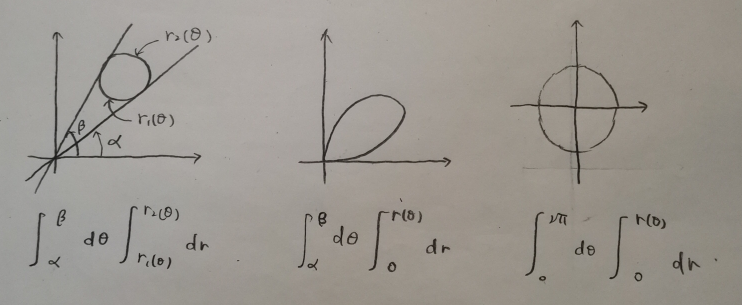
\includegraphics[width=0.8\textwidth]{二重积分极坐标换元.png}
  \caption{二重积分极坐标换元}
\end{figure}

~

\begin{exercise}[规则极坐标与广义极坐标]
  (1)计算$I = \iint_D \frac{\mathrm{d} x \mathrm{d} y}{\sqrt{1 - x^2 - y^2}}$,$D$为$x^2 + y^2 \leq 1$

  (2)广义极坐标:计算$\frac{x^2}{a^2} + \frac{y^2}{b^2} + \frac{z^2}{c^2} \leq 1$的体积
\end{exercise}

\begin{solution}
  (1)答案$2\pi$

  (2)是$8$倍第一卦限积分,该区域顶面为$z = c \sqrt{1 - \frac{x^2}{a^2} - \frac{y^2}{b^2}}$,底面为
  \begin{equation*}
    D = \left\{ (x,y) : 0 \leq y \leq b \sqrt{1 - \frac{x^2}{a^2}}, 0 \leq x \leq a \right\}
  \end{equation*}
  因此$V = 8 \iint_D c \sqrt{1 - \frac{x^2}{a^2} - \frac{y^2}{b^2}}\mathrm{d} x \mathrm{d} y$,
  利用广义极坐标变换得到$z = c \sqrt{1 - r^2}$,
  故
  \begin{equation*}
    V = 8 \int_{0 }^{\frac{\pi}{2}} \mathrm{d} \theta \int_0^1 c \sqrt{1 - r^2}abr \mathrm{d} r = \frac{4\pi}{3}abc
  \end{equation*}
\end{solution}


~

\begin{exercise}[几道非规则边界]
  (1)$f$为连续函数,将$I = \iint_D f(\frac{y}{x})\mathrm{d}x \mathrm{d} y$转化为定积分,
  其中$D: \frac{1}{4} \leq x^2 + y^2 \leq x$。

  (2)将$I = \iint_D f(x,y)\mathrm{d} x \mathrm{d} y$化为极坐标形式,其中$D : [0,1] \times [0,1]$
\end{exercise}

\begin{solution}
  (1)考虑$x = r\cos \theta, y = r\sin \theta$,
  则$\frac{1}{4} \leq r^2 \leq r \cos \theta$,
  即$\frac{1}{2} \leq r \leq \cos \theta$,
  因此$- \frac{\pi}{3} \leq \theta \leq \frac{\pi}{3}$。
  即$I = \int_{-\frac{\pi}{3}}^{\frac{\pi}{3}} \mathrm{d} \theta \int_{\frac{1}{2}}^{\cos \theta} f(\tan \theta)r\mathrm{d}r = \frac{1}{2}\int_{-\frac{\pi}{3}}^{\frac{\pi}{3}}f(\tan \theta)(\cos^2 \theta - \frac{1}{4})\mathrm{d} \theta$

  (2)一般都是先$r$后$\theta$,
  将$D$分为左上,右下两个三角形,
  则
  \begin{equation*}
    I = \int_0^{\frac{\pi}{4}} \mathrm{d} \theta \int_0^{\frac{1}{\cos \theta}} f(r \cos \theta, r\sin\theta)r\mathrm{d}r + \int_{\frac{\pi}{4}}^{\frac{\pi}{2}} \mathrm{d} \theta \int_0^{\frac{1}{\sin\theta}} f(r\cos\theta, r\sin\theta)r\mathrm{d}r 
  \end{equation*}
  先$\theta$后$r$会比较麻烦
\end{solution}

~

\noindent \textbf{三类特殊的圆}

\begin{theorem}[三类特殊圆极坐标]
  设$a > 0$,极坐标$x = r\cos \theta, y = r \sin \theta$,以下特殊圆的极坐标公式:
  \begin{itemize}
  \item $(x - a)^2 + y^2 = a^2$,即$x^2 + y^2 = 2ax$,则$r = 2a \cos \theta, \theta \in [-\frac{\pi}{2}, \frac{\pi}{2}]$
  \item $x^2 + (y-a)^2 = a^2$,即$x^2 + y^2 = 2ay$,则$r = 2a \sin \theta, \theta \in [0,\pi]$
  \item $(x - a)^2 + (y-a)^2 = 2a^2$,即$x^2 + y^2 = 2a(x+y)$,则$r = 2a(\cos \theta + \sin\theta), \theta \in [-\frac{\pi}{4}, \frac{3\pi}{4}]$
  \end{itemize}
\end{theorem}

\begin{figure}[htp]
  \centering
  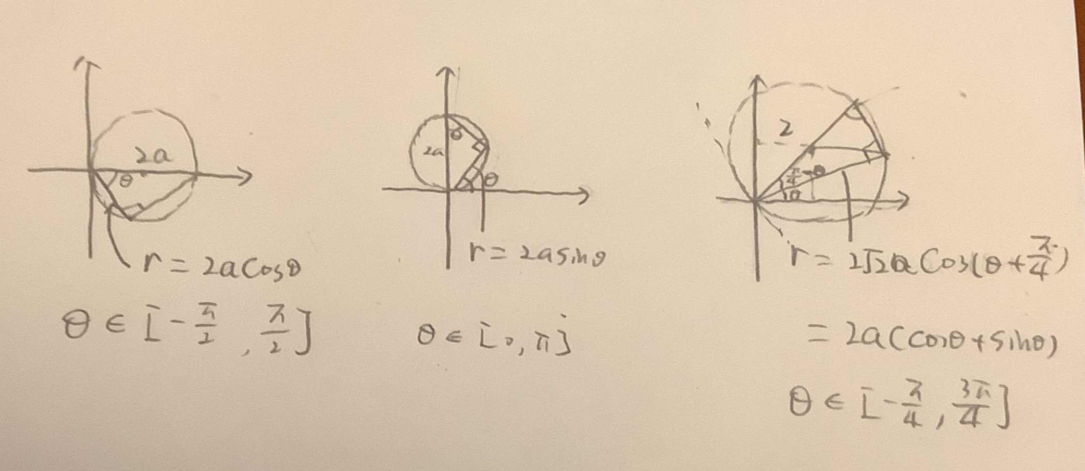
\includegraphics[width=0.6\textwidth]{二重积分三个特殊的圆.png}
  \caption{三个特殊的圆}
\end{figure}




% \subsection{广义极坐标变换}

\section{三重积分}

\subsection{投影法}

将三重积分转换为累次积分进行计算,常用的方法有投影法与截面法

\begin{theorem}[投影法]
  积分区域$V \subset \mathbb{R}^3$,
  对应$x,y$坐标平面投影区域$D$,
  且$V = \{(x,y,z):(x,y) \in D, z_1(x,y) \leq z \leq z_2(x,y)\}$,
  则:
  \begin{equation*}
    \iiint _V f(x,y,z) \mathrm{d}V = \iint _D \mathrm{d}x \mathrm{d}y \int _{z_1(x,y)}^{z_2(x,y)}f(x,y,z)\mathrm{d}z
  \end{equation*}
\end{theorem}

\begin{note}
  一般而言投影法比截面法更常用一点
\end{note}

~

\begin{exercise}[投影法]
  (1)计算$I = \iiint_V(x+y+z)\mathrm{d} V$,其中$V$是$x+y+z = 1$与坐标面围成的区域

  (2)计算$\iiint_V (x^2 + y^2 + z)\mathrm{d}V$,其中$V$是$
  \begin{cases}
    z = y\\
    x = 0
  \end{cases}
  $绕着$z$轴旋转一圈而成的曲面与$z = 1$围成的区域
\end{exercise}

\begin{solution}
  (1)用投影法$I = \iint_D \mathrm{d} x \mathrm{d} y \int_0^{1 - x- y}x+y+z \mathrm{d} z = \frac{1}{8}$

  (2)旋转面为$z = \sqrt{x^2 + y^2}$(画个图就看得出来),
  投影为$x^2 + y^2 \leq 1$,因此积分为
  \begin{align*}
    I &= \iint_D \mathrm{d} x \mathrm{d} y \int_{\sqrt{x^2 + y^2}}^1 (x^2 + y^2 + z)\mathrm{d} z \\
    &= \iint_D (x^2 + y^2)(1 - \sqrt{x^2 + y^2})\mathrm{d} x\mathrm{d} y + \frac{1}{2}\iint_D [1 - (x^2 + y^2)]\mathrm{d} x\mathrm{d} y\\
    &= \int_0^{2\pi} \mathrm{d} \theta \int_0^1 r^3 (1 - r)\mathrm{d} r + \frac{1}{2} \int_0^{2\pi}\mathrm{d} \theta \int_0^1 (1 - r^2)r\mathrm{d}r\\ 
    &= \frac{\pi}{10} + \frac{\pi}{4} = \frac{7\pi}{20}
  \end{align*}
\end{solution}

\subsection{截面法}

\begin{theorem}[截面法]
  积分区域$V \subset \mathbb{R}^3$,
  $V$被垂直于$z$轴平面截取的平面为$D_z$,
  则
  \begin{equation*}
    \iiint _Vf(x,y,z) \mathrm{d}V = \int ^b_a \mathrm{d}z \iint _{D_z}f(x,y,z)\mathrm{d}x\mathrm{d}y
  \end{equation*}
\end{theorem}

\subsection{三重积分换元法}

\begin{theorem}[三重积分换元]
  若坐标替换$x = x(u,v,w),y = y(u,v,w),z = z(u,v,w)$,
  则
  \begin{equation*}
    \iiint _V f(x,y,z) \mathrm{d}x\mathrm{d}y\mathrm{d}z = \iiint_{V^{\prime}}f(x,y,z)\left|\frac{\partial (x,y,z)}{\partial(u,v,w)}\right|\mathrm{d}u\mathrm{d}v\mathrm{d}w
  \end{equation*}
  \begin{equation*}
    \left|\frac{\partial(x,y,z)}{\partial(u,v,w)}\right| = \left|
      \begin{array}{ccc}
        \frac{\partial x}{\partial u}&\frac{\partial x}{\partial v}&\frac{\partial x}{\partial w}\\
        \frac{\partial y}{\partial u}&\frac{\partial y}{\partial v}&\frac{\partial y}{\partial w} \\
                                     \frac{\partial z}{\partial u}&\frac{\partial z}{\partial v}&\frac{\partial z}{\partial w}
      \end{array}
    \right|
  \end{equation*}
\end{theorem}

\begin{note}
  一方面还是注意Jacobi行列式外面的是绝对值。
  另一方面可以先算$\frac{\partial(u,v,w)}{\partial(x,y,z)}$,
  再取倒数和绝对值计算$\left|\frac{\partial(x,y,z)}{\partial(u,v,w)}\right|$
\end{note}

\subsection{柱面坐标变换与球坐标变换}

\begin{theorem}[柱面变换]
  做$x = r\cos \theta, y = r\sin \theta, z = z$变换时,
  $J(u,v,w) = r$。
  往往确定区域:
  \begin{equation*}
    V^{\prime} = \left\{ a \leq r \leq b, c \leq \theta \leq d, \alpha(r,\theta) \leq z \leq \beta(r,\theta) \right\}
  \end{equation*}
  因此用投影法$\iint _D \mathrm{d} r \mathrm{d} \theta \int_{\alpha(r,\theta)}^{\beta(r,\theta)} z\mathrm{d} z$,
  即一般积分顺序按照$\mathrm{d}z,\mathrm{d}r, \mathrm{d}\theta$
\end{theorem}

~

\begin{exercise}[柱坐标变换]
  (1)计算$I = \iiint_V (x^2 + y^2)\mathrm{d}V$,其中$V$是由曲面$2(x^2 + y^2) = z$与$z = 4$为界面的区域。
\end{exercise}

\begin{solution}
  (1)为抛物面与平面围成的区域,
  令$x = r \cos \theta, y = r \sin \theta, z = z$得到区域为
  \begin{equation*}
    V^{\prime} = \left\{ (r,\theta,z): 0 \leq r \leq 2, 0 \leq \theta \leq 2\pi, 2r^2 \leq z \leq 4 \right\}
  \end{equation*}
  对应积分$\iiint_{V^{\prime}} r^2 \cdot r \mathrm{d}V = \int_0^{2\pi}\mathrm{d} \theta \int_0^{\sqrt{2}}\mathrm{d} r \int_{2r^2}^4r^3\mathrm{d}z = \frac{8\pi}{3}$
\end{solution}

~

\begin{theorem}[球坐标变换]
  做$x = r \sin \varphi \cos \theta, y = r \sin \varphi \sin \theta, z = r \cos \varphi$时
  $J = r^2 \sin \varphi$。积分时先按照$\mathrm{d}r,\mathrm{d}\varphi, \mathrm{d}\theta$顺序积分
\end{theorem}


\begin{figure}[htp]
  \centering
  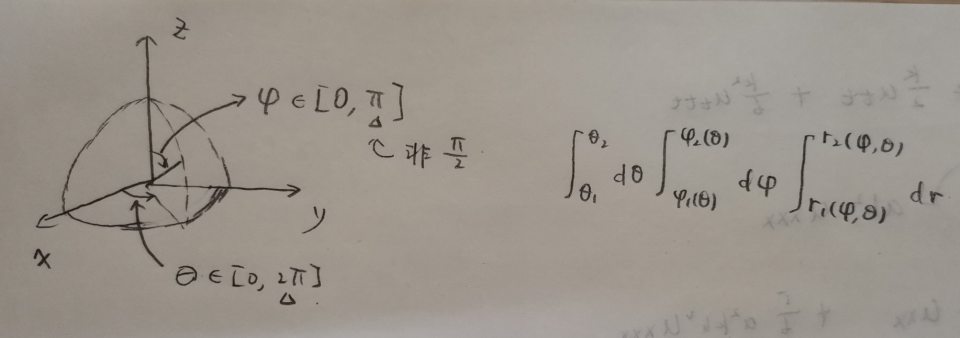
\includegraphics[width=0.8\textwidth]{三重积分极坐标换元.png}
  \caption{三重积分球坐标换元}
\end{figure}

\begin{note}
  使用球坐标变换的原则:(1)被积函数为$f(x^2 + y^2 + z^2),f(x^2+y^2)$(2)积分区域为球、锥或者其一部分
\end{note}

~

\begin{theorem}[广义球坐标变换]
  对于以$(x_0,y_0,z_0)$,以$a,b,c$为半轴长的椭球面所围成的区域$V$,
  做如下广义球坐标变换:
  \begin{equation*}
    T:
    \begin{cases}
      x = x_0 + ar \sin \varphi \cos \theta\\
      y = y_0 + br \sin \varphi \sin \theta\\
      z = z_0 + cr \cos \varphi
    \end{cases} , \quad r \geq 0, \varphi \in [0,\pi], \theta \in [0,2\pi]
  \end{equation*}
  得到
  \begin{equation*}
    |J| = \frac{\partial(x,y,z)}{\partial(r,\varphi,\theta)} = abcr^2 \sin \varphi
  \end{equation*}
\end{theorem}

~

\begin{exercise}[广义球坐标变换]
  (1)计算$I = \iiint_V z \mathrm{d} x \mathrm{d} y \mathrm{d} z$,
  其中$V$是$\frac{x^2}{a^2} + \frac{y^2}{b^2} + \frac{z^2}{c^2} \leq 1$与$z \geq 0$围成的区域
\end{exercise}

\begin{solution}
  (1)做球坐标变换,积分变为:
  \begin{equation*}
    \iiint_{V^{\prime}} cr\cos \varphi \cdot abcr^2 \sin \varphi \mathrm{d} r \mathrm{d} \varphi \mathrm{d} \theta = abc^2 \int_0^{\frac{\pi}{2}}\mathrm{d} \varphi \int_0^{2\pi} \mathrm{d} \theta \int_0^1 r^3 \sin \varphi \cos \varphi \mathrm{d} r = \frac{\pi}{4}abc^2
   \end{equation*}
\end{solution}


\newpage

\chapter{曲线积分}

\section{曲线的参数化}




\section{第一型曲线积分}

\subsection{第一型曲线积分的基本概念}

\begin{definition}[第一型曲线积分]
  $\Gamma$是$\mathbb{R}^3$中的可求长曲线,
  $f: \Gamma \rightarrow \mathbb{R}$,
  将$\Gamma$划分为分段$s_1,\cdots,s_n$,
  每段的弧长为$\Delta s_i$,
  $\xi_i = (x_i,y_i,z_i) \in s_i$,
  定义
  \begin{equation*}
    \int _{\Gamma}f(x,y,z)\mathrm{d}s = \lim \limits _{\Delta s_i \rightarrow 0} \sum\limits_{i = 1}^n f(x_i,y_i,z_i) \Delta s_i 
  \end{equation*}
\end{definition}

\begin{theorem}[第一型曲线积分的计算]
  $\Gamma$是$\mathbb{R}^3$中的光滑曲线,
  且曲线可表示为$\mathbf{r} = x(t)\mathbf{i} + y(t)\mathbf{j} + z(t)\mathbf{k}, t \in [a,b]$,
  则曲线积分为
  \begin{equation*}
    \int _{\Gamma}f(x,y,z) \mathrm{d}s = \int^b_af(x(t),y(t),z(t)) \sqrt{x^{\prime 2}(t) + y^{\prime 2}(t) + z^{\prime 2}(t)}\mathrm{d}t 
  \end{equation*}
\end{theorem}

\begin{proof}
  设$\Gamma$上的分点对应$\mathbf{r}_0,\mathbf{r}_1,\cdots,\mathbf{r}_n$,
  对应$a = t_0 < t_1 <\cdots < t_{n-1} < t_n = b$。
  首先根据弧长公式得到$\Delta s_i = \int ^{t_i}_{t_{i-1}}\sqrt{x^{\prime 2}(t) + y^{\prime 2}(t) + z^{\prime 2}(t)} \mathrm{d}t$,
  根据积分中值定理得到$\Delta s_i = \sqrt{x^{\prime 2}(\zeta_i) + y^{\prime 2}(\zeta_i) + z^{\prime 2}(\zeta_i)} \Delta t_i, \zeta_i \in [t_{i-1},t_i]$,
  代入第一型曲线积分的定义得到$\int _{\Gamma}f(x,y,z)\mathrm{d}s = \lim \limits _{||T|| \rightarrow 0} \sum\limits_{i = 1}^n f(x_i,y_i,z_i) \sqrt{x^{\prime 2}(\zeta_i) + y^{\prime 2}(\zeta_i) + z^{\prime 2}(\zeta_i)} \Delta t_i$,
  当$\Delta t_i \rightarrow 0$时即Riemann积分,
  因此得到结论。
\end{proof}

\begin{corollary}[二维第一型曲线积分的计算]
  对于$\Gamma \subset \mathbb{R}^2$,
  若平面曲线$\Gamma$可表示为$y = \varphi(x)$,
  $\varphi$在$[a,b]$连续,
  则
  \begin{equation*}
    \int _{\Gamma} f(x,y)\mathrm{d}s = \int ^b_a f(x,\varphi(x)) \sqrt{1 + \varphi^{\prime 2}(x)}\mathrm{d}x
  \end{equation*}
\end{corollary}

\begin{note}
  第一型曲线积分没有方向一说,
  例如$A,B$曲线上参数$t \in [a,b]$,
  那么积分时$AB$和$BA$的积分都是$\int_a^bf(x,y) \mathrm{d} t$,
  不能写为$\int_b^a f(x,y) \mathrm{d} t$
\end{note}

~

\begin{exercise}[极坐标格式]
  (1)$L:x^2 + y^2 = 1$,求$\int_L(x^2 + y^2)\mathrm{d} s, \int_L(x^2 + 2y^2)\mathrm{d} s$

  (2)$\int_L \sqrt{2y^2 + z^2}\mathrm{d} s$,其中$L$是$x^2 + y^2 + z^2 = a^2$与$x = y$相交的圆周

  (3)$\int_L (x^2 + y^2 + z^2)\mathrm{d} s$,这里$L$是螺旋线$x = a \cos t, y = a \sin t, z = bt$,
  $t \in [0,2\pi]$的一段

  (4)积分较难算:$\int_L xy \mathrm{d} s$,其中$L$为$\frac{x^2}{a^2} + \frac{y^2}{b^2} = 1$在第一象限的部分
\end{exercise}

\begin{solution}
  (1)$\int_L(x^2 + y^2)\mathrm{d} s = \int _L 1\mathrm{d} s = 2\pi$。
  记$x = \cos \theta, y = \sin \theta$,
  此时$(x^{\prime}(\theta))^2 + (y^{\prime}(\theta))^2 = 1$,
  因此$\int_L(x^2 + 2y^2)\mathrm{d} s = \int_0^{2\pi}(1 + \sin^2 \theta) \mathrm{d} \theta = 2\pi + 4 \cdot \frac{1}{2} \cdot \frac{\pi}{2} = 3\pi$

  (2)显然$2y^2 + z^2 = a^2$,
  因此$\int_L \sqrt{2y^2 + z^2}\mathrm{d} s = a \cdot 2a\pi = 2\pi a^2$

  (3)$x^2 + y^2 + z^2 = a^2 + b^2t^2$,
  $(x^{\prime})^2 + (y^{\prime})^2 + (z^{\prime})^2 = a^2 + b^2$,
  因此$I = \int_0^{2\pi}(a^2 + b^2t^2)\sqrt{a^2 + b^2}\mathrm{d} t = \sqrt{a^2 + b^2} (2\pi a^2 + \frac{8}{3}\pi^3 b^2)$

  (4)令$x = a \cos t, y = b \sin t$,则
  $\int_L xy \mathrm{d} s = ab \int_0^{\frac{\pi}{2}} \sin \theta \cos \theta \sqrt{a^2 \sin^2 \theta + b^2 \cos^2 \theta}\mathrm{d} \theta$,
  可化简为:
  \begin{equation*}
    \frac{ab}{2(a^2 - b^2)} \int_0^{\frac{\pi}{2}} \sqrt{(a^2 - b^2)\sin^2 \theta + b^2} \mathrm{d} [(a^2 - b^2)\sin^2 \theta] = \frac{ab(a^2 + ab + b^2)}{3(a+b)}
  \end{equation*}
\end{solution}

~

\begin{exercise}[折线形式]
  (1)计算$\int_L y \mathrm{d} s$,这里$L$为$y^2 = 4x$从$(0,0)$到$(1,2)$的一段
  
  (2)计算$\int_L (x+y) \mathrm{d} s$,这里$L$是以$O(0,0),A(1,0), B(0,1)$为顶点的三角形
\end{exercise}

\begin{solution}
  (1)$x = \frac{1}{4}y^2, y \in [0,2]$,
  因此$\int_L y \mathrm{d} s = \int_0^2 y \sqrt{1 + \frac{1}{4}y^2}\mathrm{d} y = \frac{4}{3}(2 \sqrt{2} - 1)$
  
  (2)分三段进行考虑。
  $\int_{OA}(x+y)\mathrm{d} s = \int_0^1 (x)\mathrm{d} x = \frac{1}{2}$,
  $\int_{OB}(x+y)\mathrm{d} s = \frac{1}{2}$。
  $AB$上$y = 1 - x, x \in [0,1]$,
  因此$\int_{AB}(x+y)\mathrm{d} s = \int_0^1 1 \sqrt{1 + 1}\mathrm{d} x = \sqrt{2}$,
  结果为$1 + \sqrt{2}$
\end{solution}

\subsection{使用对称性}

\begin{exercise}[镜面对称性]
  (1)计算$\int_Lxy \mathrm{d} s$,其中$L$为上半椭圆$\frac{x^2}{a^2} + \frac{y^2}{b^2} = 1( y \geq 0)$

  (2)重要:计算$\int_L |y|\mathrm{d} s$,其中$L$为双纽线$(x^2 + y^2)^2 = a^2(x^2 - y^2)$

  (3)计算$\oint_L |x|^{\frac{1}{3}} \mathrm{d} s$,这里$L$为星形线$x^{\frac{2}{3}} + y^{\frac{2}{3}} = a^{\frac{2}{3}}$
\end{exercise}

\begin{solution}
  (1)由于$L$关于$y$轴对称,而$xy$关于$y$轴对称,因此$\int_L xy\mathrm{d} s = 0$

  (2)显然$L$关于$x,y$轴均对称,
  因此将$L$分为四段,设$L_1$是第一象限的部分,
  因此$\int_L |y|\mathrm{d} s = 4 \int_{L_1}y \mathrm{d} s$,
  考虑$x = r \cos \theta, y = r \sin \theta$,
  则$L$极坐标方程为$r^2 = a^2 \cos 2\theta$,
  $L_1$方程为$r = a \sqrt{\cos 2\theta}$,且$\theta \in [0, \frac{\pi}{4}]$,即:
  \begin{equation*}
    4\int_{L_1}y\mathrm{d} s = 4 \int_0^{\frac{\pi}{4}} a \sqrt{\cos 2\theta} \sin \theta \sqrt{a^2 \cos 2\theta + a^2 \frac{\sin^2 2\theta}{\cos 2\theta}} \mathrm{d} \theta = 4 a^2 \int_0^{\frac{\pi}{4}} \sin \theta \mathrm{d} \theta = (4 - 2 \sqrt{2})a^2
  \end{equation*}

  (3)显然关于$x,y$轴对称,
  因此$\int_L|x|^{\frac{1}{3}}\mathrm{d} s = 4 \int_{L_1}x^{\frac{1}{3}}\mathrm{d} s$。
  设$x = a\cos ^3\theta, y = a \sin^3\theta, \theta \in [0,\frac{\pi}{2}]$,
  此时$x^{\prime 2}y^{\prime 2} = 9a^2 \sin^2 \cos^2 \theta$,
  结果为:
  \begin{equation*}
    I = 4\int_{L_1}x^{\frac{1}{3}} \mathrm{d} s = 12a^{\frac{4}{3}}\int_0^{\frac{\pi}{2}} \cos^2\theta \sin \theta \mathrm{d} \theta = 4a^{\frac{4}{3}}
  \end{equation*}
\end{solution}

~

\begin{exercise}[轮换对称性]
  (1)$L$是$x+y+z = 0, x^2 + y^2 + z^2 = 1$的交线,
  计算$\int_Lx \mathrm{d} s, \int_Lx^2 \mathrm{d} s, \int_Lyz \mathrm{d} s$的值

  (2)$L$是$x+y+z = 0, x^2 + y^2 + z^2 = 1$的交线,
  计算$\int_L x^2 + yz\mathrm{d} s$
\end{exercise}

\begin{solution}
  (1)考虑轮换对称性,查看交线,发现$x,y,z$轴都等价,因此变量可以随意轮换
  \begin{equation*}
    \begin{cases}
      \int_Lx\mathrm{d} s = \frac{1}{3}\int_L x+y+z \mathrm{d} s = 0\\
      \int_Lx^2 \mathrm{d} s = \frac{1}{3} \int_L x^2 + y^2 + z^2 \mathrm{d} s = \frac{1}{3} \cdot 2\pi = \frac{2\pi}{3}
    \end{cases}
  \end{equation*}
  第三个:由于$(x+y+z) = 0$,因此$(x+y+z)^2 = 0$,
  得到$(x+y+z)^2 - (x^2 + y^2 + z^2) = 2(xy + yz + xz) = -1$,即$xy + yz + xz = - \frac{1}{2}$,
  因此:
  \begin{equation*}
    \int_Lyz \mathrm{d} s = \frac{1}{3}\int_L xy + yz + xz \mathrm{d} s = \frac{1}{3} \cdot -\frac{1}{6} \cdot 2\pi = -\frac{\pi}{3}
  \end{equation*}

  (2)和第一题本质一样
\end{solution}

\subsection{曲线积分中值问题}

\begin{theorem}[曲线积分中值定理]
  $f(x,y)$是光滑曲线$L:x = x(t),y = y(t), t \in [a,b]$上的连续函数,
  设$\Delta L$是曲线$L$的弧长,
  则$\exists (x_0,y_0) \in L$,使得
  \begin{equation*}
    \int_Lf(x,y)\mathrm{d} s = f(x_0,y_0)\Delta L
  \end{equation*}
\end{theorem}

\begin{proof}
  根据计算公式得到$\int_Lf(x,y)\mathrm{d} s = \int_a^b f(x(t),y(t))\sqrt{(x^{\prime}(t))^2 + (y^{\prime}(t))^2}\mathrm{d} t$,
  根据积分第一中值定理得到等于
  $f(x(t_0),y(t_0)) \int_a^b \sqrt{(x^{\prime}(t))^2 + (y^{\prime}(t))^2}\mathrm{d} t = f(x_0,y_0) \Delta L$,
  这里$(x_0,y_0) = (x(t_0),y(t_0))$
\end{proof}

~

\begin{exercise}[积分第一中值定理的曲线推广]
  $f(x,y,z),g(x,y,z)$在可求长连续曲线$L:x = x(t),y = y(t), z = z(t), t \in [a,b]$(曲线不一定光滑!),
  上连续,且$g(x,y,z)$非负,证明:
  $\exists (\xi,\eta,\zeta) \in L$使得
  \begin{equation*}
    \int_Lf(x,y,z)g(x,y,z)\mathrm{d} s = f(\xi,\eta,\zeta) \int_Lg(x,y,z)\mathrm{d} s
  \end{equation*}
\end{exercise}

\begin{proof}
  由于不一定光滑,因此不能用含参形式计算。
  由于$f(x,y,z)$连续,设在$L$上$m \leq f(x(t),y(t),z(t)) \leq M$,
  由于$g$非负,因此$m g(x,y,z) \leq f(x,y,z) g(x,y,z) \leq M g(x,y,z)$,
  两侧积分得到:
  \begin{equation*}
    m \int_L g(x,y,z) \mathrm{d} s \leq \int_L f(x,y,z) g(x,y,z ) \mathrm{d} s \leq M \int_L g(x,y,z) \mathrm{d} s
  \end{equation*}
  若$\int_Lg(x,y,z) \mathrm{d} s = 0$,则全部为零,$(\xi,\eta,\zeta)$任选。
  若不为$0$,则同除以$\int_Lg(x,y,z)\mathrm{d} s$,得到$m \leq \frac{\int_Lf(x,y,z)g(x,y,z)\mathrm{d} s}{\int_L f(x,y,z)\mathrm{d} s} \leq M$,
  根据连续性介值性定理可证。
\end{proof}

\section{第二型曲线积分}

\subsection{基本概念与参数计算}

\begin{definition}[第二型曲线积分]
  $\Gamma$是$\mathbb{R}^3$中的有向曲线,
  其端点为$A,B \in \mathbb{R}^3$,
  $F(x,y,z) = P(x,y,z)\mathbf{i} + Q(x,y,z)\mathbf{j} + R(x,y,z)\mathbf{k}$,
  将$\Gamma$划分为$A = \mathbf{r}_0 \rightarrow \mathbf{r}_1 \rightarrow \mathbf{r}_{n-1} \rightarrow \mathbf{r}_n = B$,
  第二型曲线积分定义为:
  \begin{equation*}
    \int _{\Gamma}P\mathrm{d}x + Q\mathrm{d}y + R\mathrm{d}z = \lim \limits _{||T|| \rightarrow 0}P(\xi_i,\eta_i,\zeta_i)\Delta x_i + Q(\xi_i,\eta_i,\zeta_i)\Delta y_i + R(\xi_i,\eta_i,\zeta_i) \Delta z_i
  \end{equation*}
\end{definition}


\begin{theorem}[第二型曲线积分的计算]
  若曲线$\Gamma$由$\mathbf{r}(t) = x(t) \mathbf{i} + y(t) \mathbf{j} + z(t) \mathbf{k}, t \in [a,b]$给出,
  则
  \begin{equation*}
    \int _{\Gamma}P \mathrm{d}x + Q \mathrm{d}y + R \mathrm{d}z = \int ^b_a [P x^{\prime}(t) + Q y^{\prime}(t) + R z^{\prime}(t)]\mathrm{d}t
  \end{equation*}
\end{theorem}

~

\begin{exercise}[折线积分]
  (1)计算$\int_L x\mathrm{d} y - y\mathrm{d} x$,其中$L$为三角形$O(0,0), A(1,0),B(1,2)$为顶点的三角形逆时针曲线

  (2)计算$\int_Lx \mathrm{d} x + y\mathrm{d} y + z\mathrm{d} z$,其中$L$是$(1,1,1)$到$(2,3,4)$的直线段
\end{exercise}

\begin{solution}
  (1)分三段计算:$\int_{OA} x\mathrm{d} y - y\mathrm{d} x = 0$。
  $\int_{AB}x\mathrm{d} y - y\mathrm{d} x$以$y$为参数,
  即$\int_0^2 1 \mathrm{d} y - y \cdot 0 = 2$。
  $\int_{BO}x\mathrm{d} y -y\mathrm{d}x$,以$x$为参数,
  $y = 2x$,即$\int_1^0 x \cdot 2 - 2x \mathrm{d} x = 0$,
  最终结果为$2$。

  (2)以$x$为参数,$y = 2x - 1, z = 3x - 2$,
  因此结果为$\int_1^2 x + 2(2x - 1) + 3(3x - 2)\mathrm{d} x = 13$
\end{solution}

~

\begin{exercise}[椭圆、圆周积分]
  (1)计算$\int_L(x^2 + 2xy)\mathrm{d} y$,其中$L$为$\frac{x^2}{a^2} + \frac{y^2}{b^2} = 1(y \geq 0)$方向逆时针

  (2)计算$I = \oint _L \frac{-x \mathrm{d} x + y\mathrm{d} y}{x^2 + y^2}$,其中$L$为圆周$x^2 + y^2 = 1$,方向逆时针
\end{exercise}

\begin{solution}
  (1)设$x = a \cos \theta, y = b \sin \theta, \theta \in [0,\pi]$。
  则$\int_L (x^2 + 2xy)\mathrm{d} y = \int_0^{\pi} a^2 \cos^3\theta + 2ab^2 \sin \theta \cos^2\theta \mathrm{d} \theta = \frac{4}{3}ab^2$

  (2)设$x = \cos \theta, y = \sin \theta, \theta \in [0,2\pi]$,
  则$I = \int_0^{2\pi}(\cos \theta \sin \theta + \sin \theta \cos \theta)\mathrm{d} \theta = 0$
\end{solution}

~

\begin{exercise}[交线积分:化为单变量]
  (1)计算$I = \oint _L (y-z)\mathrm{d} x + (z - x)\mathrm{d} y + (x - y)\mathrm{d}z$,
  其中$L$为$x^2 + y^2 = 1, x + z = 1$,从$z$轴正无穷看为顺时针

  (2)重要:计算$\oint_L xyz \mathrm{d} z$,其中$L$为$x^2 + y^2 + z^2 = 1$与$y = z$相交的圆,
  方向为$1,2,7,8$卦限。
\end{exercise}

\begin{solution}
  (1)设$x = \cos \theta, y = \sin \theta, z = 1 - \cos \theta$,
  则$\theta \in [2\pi,0]$(不是$[0,2\pi]$!)。
  则
  \begin{equation*}
    I = \int_{2\pi}^0 [(\sin \theta + \cos \theta - 1)(-\sin \theta) + (1 - 2\cos \theta)\cos \theta + (\cos \theta - \sin \theta)\sin\theta]\mathrm{d} \theta = 4\pi
  \end{equation*}

  (2)由于$x^2 + 2y^2 = 1$,设$x = \cos \theta, y = z = \frac{1}{\sqrt{2}}\sin \theta$,
  由于从第一卦限出发,$x,y,z$均为正,而$\theta$为小正数时,位于第一卦限,因此$\theta \in [0,2\pi]$。
  因此:
  \begin{equation*}
    I = \int_0^{2\pi} \frac{1}{2}\cos \theta \sin ^2 \theta \frac{1}{\sqrt{2}} \cos \theta \mathrm{d} \theta = \frac{\sqrt{2}\pi}{16}
  \end{equation*}
\end{solution}

\begin{note}
  第二题虽然是球面的一部分,但是曲线积分都要化成一个变量的,
  因此不能用球坐标变换!
\end{note}

~

\begin{exercise}[二次曲面交线]
  计算$\int_L y\mathrm{d} x + z\mathrm{d} y + x \mathrm{d} z $,其中$L$为椭球与柱面交线:
  \begin{equation*}
    \frac{x^2}{a^2} + \frac{y^2}{b^2} + \frac{z^2}{c^2} = 1, \frac{x}{a} + \frac{z}{c} = 1, x,y,z \geq 0
  \end{equation*}
  方向从$(a,0,0)$到$(0,0,c)$
\end{exercise}

\begin{solution}
  (1)直接用极坐标极度不方便,
  先令$x = a\overline{x}, y = b\overline{y}, z = c\overline{z}$,
  得到$\overline{x}^2 + \overline{y}^2 + \overline{z}^2 = 1, \overline{x} + \overline{z} = 1$。
  将前者配凑为$(\overline{x} + \overline{z})^2 + (\overline{x} - \overline{z})^2 + 2\overline{y}^2 = 2$,
  因此$(\overline{x} - \overline{z})^2 + 2\overline{y}^2 = 1$,
  因此设$\overline{x} - \overline{z} = \cos \theta, \sqrt{2}\overline{y} = \sin \theta$,
  得出$\overline{x} = \frac{1}{2} (1 + \cos \theta), \overline{y} = \frac{1}{\sqrt{2}}\sin \theta, \overline{z} = \frac{1}{2}(1 - \cos \theta)$,
  根据方向以及端点可判断$\theta \in [0,\pi]$(具体含义难以判断)。
  因此代入计算可知结果为$\frac{ac}{2} - \frac{\pi b}{4 \sqrt{2}} (a + c)$
\end{solution}


\subsection{使用对称性}

和第一型曲线积分一样,下面考虑镜像对称以及轮换对称性

\begin{itemize}
\item 镜像对称:如$\int_S f(x,y,z)\mathrm{d} x$,要同时考虑$f(x,y,z)$和$\mathrm{d} x$在$S$上的符号
\item 轮换对称:要保证积分区域和积分表达式均轮换对称。
  轮换有两种使用方法:(1)保持积分区域不变,积分表达式轮换
  (2)保持积分表达式不变,积分区域轮换(具体见轮换对称练习)
\end{itemize}

\begin{theorem}[$\mathrm{d}x$的符号]
  若沿着给定方向,$x$由大变小,则$\mathrm{d} x$为负,同理若变大则$\mathrm{d} x$为正,
  以此判断对称性。
  如果不容易直接判断,则画出投影曲线,再在平面曲线上判断方向。
\end{theorem}

~

\begin{exercise}[镜像对称性]
  (1)证明$I = \oint _L \frac{-x\mathrm{d} x + y\mathrm{d} y}{x^2 + y^2} = 0$,
  其中$L$为圆周$x^2 + y^2 = 1$,方向逆时针。

  (2)计算$I = \int_L (-2xe^{-x^2} \sin y)\mathrm{d} x + (e^{-x^2} \cos y + x^4 )\mathrm{d} y$,
  其中$L$为$(1,0)$到$(-1,0)$的半圆$y = \sqrt{1 - x^2}$
\end{exercise}

\begin{solution}
  (1)$I = - \int_L x\mathrm{d} x + \int_L y\mathrm{d} y$,
  前者分为$x$轴上下两部分,上下$x$符号大小均相等,由于上方$x$从大变小,下方从小变大,因此$\mathrm{d} x$符号相反,
  得到$- \int_L x \mathrm{d} x = 0$。
  后者同理根据$x$轴上下两部分得到结果为$0$。

  (2)关于$y$轴对称。
  第一项$\mathrm{d} x$同号,$-2xe^{-x^2}\sin y$异号,因此第一个积分为$0$。
  第二个$\mathrm{d} y$异号,$e^{-x^2}\cos y + x^4$同号等值,因此第二个积分也为$0$。
  综上整个积分为$0$。
\end{solution}

~

\begin{exercise}[轮换对称性]
  (1)计算$\int_Lx\mathrm{d} x + y\mathrm{d} y + z\mathrm{d} z$,其中$L$为$x^2 + y^2 + z^2 = 1$与$x+y+z = 0$相交圆周,
  $L$从第一卦限来看是逆时针的。

  (2)计算$\int_L (y^2 - z^2)\mathrm{d} x + (z^2 - x^2)\mathrm{d} y + (x^2 - y^2)\mathrm{d} z$,
  其中$L$为$x^2 + y^2 + z^2 = 1$在第一卦限的边界曲线,
  方向为$xy$平面,$yz$平面,$zx$平面
\end{exercise}

\begin{solution}
  (1)由于$x,y,z$可以随便互换,
  $I$可以写出$3 \int_L x\mathrm{d} x$或$y,z$对应积分,
  要选择一个好算的。
  考虑$z = -(x + y)$,
  则$x^2 + y^2 + (x + y)^2 = 1$,得到$(x + \frac{1}{2}y)^2 + \frac{3}{4}y^2 = \frac{1}{2}$。
  因此令$x + \frac{1}{2}y = \frac{1}{\sqrt{2}} \cos \theta, \frac{\sqrt{3}}{2}y = \frac{1}{\sqrt{2}}\sin \theta$,
  因此得到参数方程为:
  \begin{equation*}
    x = \frac{1}{\sqrt{2}} \cos \theta - \frac{1}{\sqrt{6}} \sin \theta, y = \frac{2}{\sqrt{6}}\sin \theta, z = - \frac{1}{\sqrt{2}} \cos \theta - \frac{1}{\sqrt{6}} \sin \theta, \theta \in [0,2\pi]
  \end{equation*}
  可以算$\int_L y\mathrm{d} y$比较简单,因此最终结果为$0$。

  (2)
  设三个部分曲线分别为$L_1,L_2,L_3$,
  由于$x,y,z$可以随便互换,
  若$(x,y,z) \rightarrow (z,x,y)$,则积分表达式不变,
  而$L_1$部分在该变换下变为$L_2$,因此$L_1,L_2,L_3$积分值相等。
  因此$I = 3 \int_{L_1} (y^2 - z^2)\mathrm{d} x + (z^2 - x^2)\mathrm{d} y + (x^2 - y^2)\mathrm{d} z = $,
  对于$L_1$而言,虽然积分表达式轮换对称,但是积分区域不轮换对称,因此只能硬算了。
  取$x = \cos \theta, y = \sin \theta, z = 0,\theta \in [0,\frac{\pi}{2}]$,
  得到结果为$-4$。

\end{solution}

~

\begin{exercise}[双曲面交线+对称性]
  重点:计算$I = \int_L y^2 \mathrm{d} x + z^2 \mathrm{d} y + x^2 \mathrm{d} z$,其中$L$是维维安尼曲线
  $x^2 + y^2 + z^2 = a^2, x^2 + y^2 = ax(z \geq 0, a > 0)$,
  从$x$轴$+\infty$看去,$L$方向为逆时针
\end{exercise}

\begin{solution}
  注意$x^2 + y^2 = ax$即$(x - \frac{a}{2})^2 + y^2 = \frac{a^2}{4}$是圆柱面,且过原点。
  考虑关于$xz$平面对称,
  积分表达式显然不变,
  $\mathrm{d} x$相反,$\mathrm{d} y$相同(需要把投影的圆画出来看看),$\mathrm{d} z$相反,
  因此只需要计算$I = \int_L z^2 \mathrm{d} y = 2\int_{L_1} z^2 \mathrm{d} y$,
  这里$L_1$是$L$在$y \geq 0$的部分,
  设$x = a \sin \varphi \cos \theta, y = a \sin \varphi \sin \theta, z = a \cos \varphi, \theta \in [0,\frac{\pi}{2}]$($\theta$的范围具体见三重积分球坐标变换),
  代入柱面公式得到$\sin \varphi = \cos \theta$,即$\theta = \frac{\pi}{2} - \varphi$,
  综上$L_1$的参数方程为:
  \begin{equation*}
    x = a \sin^2 \varphi, y = a \sin \varphi \cos \varphi, z = a \cos \varphi, \varphi \in [\frac{\pi}{2}, 0]
  \end{equation*}
  得到最终结果为$-\frac{\pi}{4}a^3$
\end{solution}

\subsection{两类曲线积分的关系}

\begin{theorem}[光滑曲线切向量]
  考虑光滑曲线$\mathbf{r}(s) = (x(s),y(s)), s \in [0,l]$,
  满足$(x^{\prime}(s))^2 + (y^{\prime}(x))^2 = 1$。
  则其单位切向量为$\mathbf{t} = (x^{\prime}(s), y^{\prime}(s)) = (\cos(\mathbf{t},x), \cos (\mathbf{t},y))$,
  即
  \begin{equation*}
    \mathrm{d} x = \cos (\mathbf{t},x)\mathrm{d} s, \quad \mathrm{d} y = \cos(\mathbf{t},y)\mathrm{d} s
  \end{equation*}
\end{theorem}

\begin{theorem}[两类曲线积分的关系]
  根据光滑曲线切向量的结论,可知:
  \begin{equation*}
    \int_L P\mathrm{d} x + Q\mathrm{d} y = \int_L \left[ P(x,y)\cos(\mathbf{t},x) + Q(x,y) \cos (\mathbf{t},y) \right]\mathrm{d} s
  \end{equation*}
\end{theorem}



\section{Green公式}

\subsection{Green公式及其基本应用}

\begin{theorem}[Green公式]
  $\Omega \subset \mathbb{R}^2$是有限条分段光滑曲线连接成的闭曲线,
  $P(x,y),Q(x,y)$在$\Omega$上连续,
  且有连续偏导$\frac{\partial Q}{\partial x}, \frac{\partial P}{\partial y}$,
  沿着$\partial \Omega$的方向,$\Omega$一直在左侧,
  则
  \begin{equation*}
    \int _{\partial \Omega} P\mathrm{d}x + Q \mathrm{d}y = \iint _{\Omega} (\frac{\partial Q}{\partial x} - \frac{\partial P}{\partial y})\mathrm{d}x\mathrm{d}y
  \end{equation*}
\end{theorem}

\begin{note}
  使用Green公式的基本条件是曲线光滑和偏导存在,
  一般在$P,Q$本身复杂,但$\frac{\partial Q}{\partial x} - \frac{\partial P}{\partial y}$简单时使用。
  记忆时可记忆为:
  \begin{equation*}
    \left|
      \begin{array}{cc}
        \frac{\partial }{\partial x}&\frac{\partial}{\partial y}\\
        P&Q
      \end{array}
    \right|
  \end{equation*}
\end{note}

~

\begin{exercise}[Green公式基本应用]
  (1)$a,b$为正数,$L$为从$(2a,0)$到$(0,0)$的半圆$y = \sqrt{2ax - x^2}$,
  计算
  \begin{equation*}
    I = \int_L [e^x \sin y - b(x+y)]\mathrm{d} x + (e^x \cos y - ax)\mathrm{d} y
  \end{equation*}

  (2)$L$为$\sin x$从$(0,0)$到$(\pi,0)$的一段,计算:
  \begin{equation*}
    I = \int_L \sqrt{x^2 + y^2}\mathrm{d} x + y \left[ xy + \ln \left( x + \sqrt{x^2 + y^2} \right) \right]\mathrm{d} y
  \end{equation*}

  (3)$L$为曲线$y = \sin x$从$(0,0)$到$(\pi,0)$的一段,计算
  \begin{equation*}
    I = \int_L e^x \left[ (1 - \cos y) \mathrm{d} x - (y - \sin y)\mathrm{d} y \right]
  \end{equation*}
\end{exercise}

\begin{solution}
  (1)显然积分本身很麻烦,
  考虑$P = e^x \sin y - b(x+y), Q = e^x \cos y - ax$,
  则$Q_x - P_y = b-a$很方便,因此考虑用Green公式把圆周补上,
  记$L_1$为$(0,0) \rightarrow (2a,0)$直线。
  则$I = \int_{L + L_1} - \int_{L_1} = \iint_D b - a \mathrm{d} x \mathrm{d} y - \int_{L_1} -bx \mathrm{d} x =   \frac{1}{2}\pi a^2(b-a) + 2a^2b$

  (2)考虑$Q_x - P_y = y^2 + \frac{y + \frac{xy}{\sqrt{x^2 + y^2}}}{x + \sqrt{x^2 + y^2}} - \frac{y}{\sqrt{x^2 + y^2}} = y^2$,
  记$L_1$是$(\pi,0)$到$(0,0)$的直线段,
  则$\int_L P\mathrm{d} x + Q\mathrm{d} y = \int_{\pi}^0 x\mathrm{d} x = - \frac{1}{2}\pi^2$,
  因此:
  \begin{equation*}
    I = \int_{L+L_1} - \int_{L_1} = - \iint_D y^2\mathrm{d} x \mathrm{d} y + \frac{1}{2}\pi^2 = - \int_0^{\pi}\mathrm{d} x \int_0^{\sin x}y^2 \mathrm{d} y + \frac{1}{2}\pi^2 = \frac{1}{2}\pi^2 - \frac{4}{9}
  \end{equation*}

  (3)首先$Q_x - P_y = -ye^x$,记$L_1$为$(\pi,0) \rightarrow (0,0)$的直线,
  最终结果为$\frac{1}{5}(e^\pi - 1)$。
  中间$\frac{1}{2}\int_0^{\pi}e^x \sin ^2x \mathrm{d} x = \frac{1}{4}\int_0^{\pi}e^x (1 - \cos 2x)\mathrm{d} x = \frac{1}{4} e^x \bigg|_0^{\pi} - \frac{1}{4}\frac{e^x}{4+1}(\cos 2x + 2\sin 2x)\bigg|_0^{\pi}$
\end{solution}

~

\begin{exercise}[一道经典题]
  (1)计算$I = \oint _L \frac{x\mathrm{d}y - y\mathrm{d} x }{x^2 + y^2}$,其中$L$为任一不包含原点区域的边界(包含原点情况在后面讨论)。
\end{exercise}

\begin{solution}
  (1)结果为$0$
\end{solution}

~

\begin{theorem}[区域面积转换为曲线积分]
  平面区域$D$的面积为:
  \begin{equation*}
    S_D = \iint_D \mathrm{d} S = \frac{1}{2} \oint _L x\mathrm{d}y - y\mathrm{d} x
  \end{equation*}
\end{theorem}

~

\begin{exercise}[曲面面积应用]
  计算抛物线$(x+y)^2 = ax(a > 0)$与$x$轴围成的面积
\end{exercise}

\begin{solution}
  结果:$\frac{1}{6}a^2$,见华东师大课本
\end{solution}

\subsection{内部有瑕点}

\begin{theorem}[瑕点Green公式]
  若$P(x,y),Q(x,y)$除瑕点外满足$Q_x - P_y = 0$,
  边界$L$围成的区域$D$包含瑕点$x_0$,
  则可作包含$x_0$的小区域$D_1$,其边界$L_1$,方向逆时针,
  根据$\int_L - \int_{L_1} = \iint_{D - D_1} = 0$得出:
  \begin{equation*}
   \int_L P\mathrm{d} x + Q \mathrm{d} y = \int_{L_1} P \mathrm{d} x + Q \mathrm{d} y 
  \end{equation*}
  保证$L_1$曲线表达式的特殊性即可快速计算出结果。
\end{theorem}

\begin{exercise}[最经典题目]
  重点:$L$为简单封闭光滑曲线,且不经过原点,$a,b > 0$,计算$I = \oint _L \frac{x \mathrm{d} y - y\mathrm{d} x}{ax^2 + by^2}$。
\end{exercise}

\begin{solution}
  显然$P,Q$在不包含原点的区域上有连续偏导数,
  $P_y = \frac{-(ax^2 + by^2) + y \cdot 2by}{(ax^2 + by^2)^2}, Q_x = \frac{by^2 - ax^2}{(ax^2 + by^2)^2}$,
  若$L$围成的区域不包含原点,则根据$Q_x - P_y = 0$得到积分为$0$。
  若$D$包含原点,考虑挖去原点的小区域,其边界$L_1$为$ax^2 + by^2 = r^2$,方向逆时针。
  则$\int_L P \mathrm{d} x + Q \mathrm{d} y = \int_{L_1} P \mathrm{d} x + Q \mathrm{d} y = \frac{1}{r^2} \int_{L_1}x\mathrm{d} y - y\mathrm{d} x$,
  再次使用Green公式得到结果为$\frac{1}{r^2}\iint_{D_1}2 \mathrm{d} x \mathrm{d} y = \frac{2\pi}{\sqrt{ab}}$。
\end{solution}

\begin{corollary}[常用函数1]
  若$P_0(x_0,y_0)$则:
  \begin{equation*}
    \oint_L \frac{(x - x_0)\mathrm{d} y - (y - y_0)\mathrm{d} x}{a(x - x_0)^2 + b(y - y_0)^2} =
    \begin{cases}
      \frac{2\pi}{\sqrt{ab}}, &L\text{围成的区域包含}P_0\\
      0, & L\text{围成的区域不包含}P_0
    \end{cases}
  \end{equation*}
\end{corollary}

~

\begin{exercise}[推广题1]
  计算$I = \oint _L \frac{(x-y)\mathrm{d} x + (x + 4y)\mathrm{d} y}{x^2 + 4y^2}$,
  其中$L$为$x^2 + y^2 = 1$,方向逆时针
\end{exercise}

\begin{solution}
  $P_y = Q_x = \frac{-x^2 - 8xy + 4y^2}{(x^2 + 4y^2)^2}$,
  记$L_1$为$x^2 + 4y^2 = r^2$,
  则$I = \int_{L_1}P\mathrm{d} x + Q\mathrm{d} y = \frac{1}{r^2} \int_{L_1}(x - y)\mathrm{d} x + (x + 4y)\mathrm{d} y$,
  再用Green公式得到$I = \frac{1}{r^2} \iint_{D_1} 2 \mathrm{d} x \mathrm{d} y = \frac{2}{r^2} \cdot \frac{\pi r^2}{2} = \pi$
\end{solution}

\begin{corollary}[常用函数2]
  $c_1,c_2 > 0$时,$a_2 = -b_1, \frac{a_1}{c_1} = \frac{b_2}{c_2}$有:
  \begin{equation*}
    \oint_L \frac{(a_1x + a_2y)\mathrm{d}x + (b_1 x + b_2y)\mathrm{d} y}{c_1x^2 + c_2y^2} =
    \begin{cases}
      \frac{2b_1\pi}{\sqrt{c_1c_2}}, & L\text{围成区域包含原点}\\
      0, & L\text{围成区域不包含原点}
    \end{cases}
  \end{equation*}
\end{corollary}

~

\begin{lemma}[推广椭圆面积]
  设$a,c > 0, ac - b^2 > 0$,
  考虑$ax^2 + 2bxy + cy^2 = 1$,则该曲线为椭圆,
  围成的面积为$\frac{\pi}{\sqrt{ac - b^2}}$
\end{lemma}

\begin{proof}
  写为$a(x + \frac{b}{a}y)^2 + (c - \frac{b^2}{a})y^2 = 1$,
  等价于$\frac{x^2}{1/a} + \frac{y^2}{a/(ac - b^2)} = 1$,
  根据椭圆面积公式($\pi \cdot ab$)得到$\frac{\pi}{\sqrt{ac - b^2}}$
\end{proof}

\begin{exercise}[推广题2]
  重点:计算$I = \oint _L \frac{x\mathrm{d} y - y\mathrm{d} x}{x^2 + xy + y^2}$,
  $L$是圆周$x^2 + y^2 = 1$,逆时针方向。
\end{exercise}

\begin{solution}
  分母即$(x + \frac{1}{2}y)^2 + \frac{3}{4}y^2 = 0$,
  若分母为$0$,则$x = y = 0$。
  $P_y = Q_x = \frac{y^2 - x^2}{(x^2 + xy + y^2)^2}$,
  取$L_1$为$x^2 + xy + y^2= r^2$,该图形为椭圆,
  面积为$\frac{2\pi r^2}{\sqrt{3}}$,
  使用Green公式得到结果为$\frac{4\pi}{\sqrt{3}}$
\end{solution}

\begin{corollary}[常用函数3]
  若$a,b,c$满足$a, c > 0, ac - b^2 > 0$,则
  \begin{equation*}
    \oint _L \frac{x\mathrm{d} y - y\mathrm{d} x}{ax^2 + 2bxy + cy^2} = \frac{2\pi}{\sqrt{ac - b^2}}
  \end{equation*}
\end{corollary}

~

\begin{exercise}[其他形式]
  $L$为不过原点的简单光滑封闭曲线,
  计算:
  \begin{equation*}
    I = \oint_{L }\frac{e^y}{x^2 + y^2} \left[ (x \sin x + y \cos x)\mathrm{d} x + (y \sin x - x \cos x)\mathrm{d} y \right]
  \end{equation*}
\end{exercise}


\subsection{曲线积分与路径无关性}

\begin{theorem}[路径无关性]
  $D$为单连通区域,若$P(x,y),Q(x,y)$在$D$连续且有一阶连续偏导,
  $L$为$D$内任意按段光滑曲线
  则$\int_L P\mathrm{d} x + Q \mathrm{d} y$与路径无关当且仅当:
  \begin{itemize}
  \item $D$内处处有$P_y = Q_x$
  \item $D$内任意按段光滑闭合曲线$L$,有$\oint_L P \mathrm{d} x + Q \mathrm{d} y = 0$
  \item $D$内存在原函数$u(x,y)$使得$\mathrm{d} u = P \mathrm{d} x + Q \mathrm{d} y$
  \end{itemize}
\end{theorem}




\newpage

\chapter{曲面积分}

\section{曲面的面积}

\begin{theorem}[曲面面积公式]
  $D$是可求面积平面有界区域,$z = f(x,y)$在$D$上有连续一阶偏导,则曲面$z = f(x,y), (x,y) \in D$的面积为:
  \begin{equation*}
    \Delta S = \iint_D \sqrt{1 + f_x^2 + f_y^2}\mathrm{d} x\mathrm{d} y
  \end{equation*}
\end{theorem}

\begin{theorem}[参数方程曲面面积]
  $D$为可求面积平面有界区域,
  $x = x(u,v), y = y(u,v), z = z(u,v)$在$D$上有连续一阶偏导,
  则曲面$\mathbf{r}(u,v) = (x(u,v),y(u,v),z(u,v))$的面积公式为:
  \begin{equation*}
    \Delta S = \iint_D \sqrt{EG - F^2}\mathrm{d} u \mathrm{d} v,
    \begin{cases}
      E = x_u^2 + y_u^2 + z_u^2\\
      F = x_ux_v + y_uy_v + z_uz_v\\
      G = x_v^2 + y_v^2 + z_v^2
    \end{cases}
  \end{equation*}
\end{theorem}

~

\begin{exercise}[曲面面积计算]
  (1)证明$x^2 + y^2 + z^2 = R^2$的表面积为$4 \pi R^2$
\end{exercise}

\begin{solution}
  (1)考虑上半平面$z = \sqrt{R^2 - x^2 - y^2}$,
  $D$为$x^2 + y^2 \leq R^2$,
  则$z_x = - \frac{x}{z}, z_y = - \frac{y}{z}$,
  因此$\sqrt{1 + z_x^2 + z_y^2} = \frac{R}{z}$。
  得到球面面积为
  \begin{equation*}
   S =  
   2 \iint_D \frac{R}{z} \mathrm{d} x \mathrm{d} y = 2 \int_0^R \mathrm{d} r \int_0^{2\pi} \frac{R}{\sqrt{R^2 - r^2}} r \mathrm{d} \theta = 4\pi R \sqrt{R^2 - r^2} \bigg|_R^0 = 4\pi R^2
  \end{equation*}
\end{solution}

\begin{note}
  对于$x^2 + y^2 + z^2 = a^2$,
  有$\sqrt{1 + z_x^2 + z_y^2} = \frac{a}{z}$,这个结论在计算球面曲面积分时经常用到!
\end{note}

\section{第一型曲面积分}

\subsection{基本概念与计算公式}

\begin{definition}[第一型曲面积分]
  $S$为光滑曲面片,
  对$S$做分割$S = \{\Delta S_1,\cdots,\Delta S_n\}$,
  记$||\Delta|| = \max \{s(\Delta S_i)\}$,
  则定义
  \begin{equation*}
    \iint _S f(x,y,z) \mathrm{d}S = \lim \limits _{||\Delta|| \rightarrow 0}\sum\limits_{i = 1}^n f(x_i,y_i,z_i)\Delta S_i
  \end{equation*}
\end{definition}


\begin{theorem}[投影法]
  若$S$可表示为$z = z(x,y), (x,y) \in D$,
  则
  \begin{equation*}
    \iint _S f(x,y,z) \mathrm{d}S = \iint _D f(x,y,z(x,y))\sqrt{1 + (\frac{\partial z}{\partial x})^2 + (\frac{\partial z}{\partial y})^2 }\mathrm{d}x\mathrm{d}y
  \end{equation*}
\end{theorem}

\begin{theorem}[球坐标变换结论]
  对于球面$x^2 + y^2 + z^2 = a^2$,
  令$z = \sqrt{a^2 - x^2 - y^2}$,则得到
  \begin{equation*}
    \sqrt{1 + z_x^2 + z_y^2} = \frac{a}{z}
  \end{equation*}
\end{theorem}

\begin{proof}
  直接计算可验证
\end{proof}

\begin{note}
  球面可以使用投影法或极坐标,本质上两者都可以用,而且相差不大。
\end{note}

~

\begin{exercise}[投影法]
  (1)计算$\iint_S \frac{\mathrm{d} S}{z}$,其中$S$是球面$x^2 + y^2 + z^2 = a^2$被平面
  $z = h$所截的顶部。
  
  (2)计算$A = \int _S(x + y + z)\mathrm{d}S$,
  这里$S$表示$x^2 + y^2 + z^2 = a^2(z \geq 0)$,即球上表面
\end{exercise}

\begin{solution}
  (1)做投影法$z = \sqrt{a^2 - x^2 - y^2}$,
  积分变为$\iint_D \frac{a}{z^2}\mathrm{d} x \mathrm{d} y = \iint_D \frac{a}{a^2 - x^2 - y^2}\mathrm{d} x \mathrm{d} y$,
  做极坐标变换得到
  \begin{equation*}
    \int_0^{2\pi}\mathrm{d} \theta \int_0^{\sqrt{a^2 - h^2}} \frac{a}{a^2 - r^2}r\mathrm{d} r = 2\pi a \ln \frac{a}{h}
  \end{equation*}
  
  (2)根据对称性只剩一项,即$A = \iint _S z \mathrm{d}S $,
  因此根据$z = \sqrt{a^2 - x^2 - y^2}$代入计算得到:
  \begin{equation*}
    A = \iint_{x^2 + y^2 \leq a^2} z \cdot \frac{a}{z} \mathrm{d}x\mathrm{d}y= \iint_{x^2 + y^2 \leq a^2}a \mathrm{d}x\mathrm{d}y = a^3 \pi
  \end{equation*}
\end{solution}

~


\begin{theorem}[参数方程法]
  若$S$由参数方程$x(u,v),y(u,v),z(u,v)$给出,
  $(u,v) \in D$,
  则
  \begin{equation*}
    \iint _S f(x,y,z) \mathrm{d}S = \iint_D f[x(u,v),y(u,v),z(u,v)]\sqrt{EG - F^2}\mathrm{d}u\mathrm{d}v, \text{其中:}
    \begin{cases}
      E = x_u^2 + y_u^2 + z_u^2\\
      F = x_ux_v + y_uy_v + z_uz_v\\
      G = x_v^2 + y_v^2 + z_v^2
    \end{cases}
  \end{equation*}
\end{theorem}

\begin{theorem}[球坐标极坐标变换]
  对于球面$x^2 + y^2 + z^2 = a^2$,
  令$x = a \sin \varphi \cos \theta, y = a \sin \varphi \sin \theta, z = a \cos \varphi$,则
  \begin{equation*}
    \begin{cases}
      E = a^2 \sin ^2 \varphi\\
      F = 0\\
      G = a^2
    \end{cases} \Rightarrow \sqrt{EG - F^2} = a^2 \sin \varphi
  \end{equation*}
\end{theorem}

~

\begin{exercise}[参数方程法]
  (1)重点:计算$I = \iint_S \frac{\mathrm{d} S}{\sqrt{x^2 + y^2 + (z + a)^2}}$,
  其中$S$为$x^2 + y^2 + z^2 = a^2(z \geq 0)$
\end{exercise}

\begin{solution}
  (1)采用球坐标变换,积分变为$I = \iint_{S^{\prime}} \frac{a^2 \sin \varphi}{\sqrt{a^2 \sin^2 \varphi + a^2( \cos \varphi + 1)^2}}\mathrm{d} \theta \mathrm{d} \varphi$,
  区域为$\varphi \in [0, \frac{\pi}{2}], \theta \in [0,2\pi]$,
  进一步化简得到:
  \begin{equation*}
    I = \iint_{S^{\prime}}\frac{-a \sin \varphi }{\sqrt{2} \sqrt{1 + \cos \varphi}}\mathrm{d} \theta \mathrm{d} \varphi = - \sqrt{2}\pi a \int_0^{\frac{\pi}{2}} \frac{\mathrm{d}(\cos \varphi)}{\sqrt{1 + \cos \varphi}} = 4\pi a - 2 \sqrt{2} \pi a
  \end{equation*}
\end{solution}

\subsection{使用对称性}

\begin{exercise}[积分曲面对称]
  (1)计算$\iint_S(x + \sin yz)\mathrm{d} S$,其中$S$为球面$x^2 + y^2 + z^2 = a^2$

  (2)$\iint_S (x+y+z)^3 \mathrm{d} S$,其中$S$为$|x| + |y| + |z| = 1$
\end{exercise}

\begin{solution}
  (1)根据$S$关于$yz$平面对称得到$\iint_S x\mathrm{d} s = 0$,
  根据$S$关于$xz$平面对称得到$\iint _S \sin yz \mathrm{d} s = 0$

  (2)根据关于原点中心对称性得到为$0$。
\end{solution}

~

\begin{exercise}[轮换对称性]
  (1)计算$I = \iint_S x^2 \mathrm{d} S$与$J = \iint xy \mathrm{d} S$,
  其中$S$为球面$x^2 + y^2 + z^2 = a^2$
\end{exercise}

\begin{solution}
  (1)由于$S$有轮换对称性,
  得到$I = \frac{1}{3} \iint_S x^2 + y^2 + z^2 \mathrm{d} S = \frac{4}{3}\pi a^4$。
  $J$没必要考虑轮换对称性,
  由于$S$关于$yz$平面对称,因此$J = 0$。
\end{solution}




\section{第二型曲面积分}

\subsection{基本概念、投影法、参数方程法}

\begin{definition}[第二型曲面积分]
  对于向量场$F(x,y,z) = (P(x,y,z),Q(x,y,z),R(x,y,z))$,
  其通过曲面$S$的通量定义为第二型曲面积分(向外为正):
  \begin{equation*}
    \iint _S P(x,y,z)\mathrm{d}y\mathrm{d}z + Q(x,y,z)\mathrm{d}z\mathrm{d}x + R(x,y,z)\mathrm{d}x\mathrm{d}y
  \end{equation*}
\end{definition}

\begin{theorem}[投影法]
  若曲面$S$的方程为$z = z(x,y)$,在$xy$平面投影区域为$D_{xy}$,则
  \begin{equation*}
    \iint_S R(x,y,z) \mathrm{d} x \mathrm{d} y = \pm \iint_{D_{xy}} R(x,y,z(x,y))\mathrm{d} x \mathrm{d} y
  \end{equation*}
  正负取决于$S$的法向量与$z$轴正向的夹角,若锐角则取正,钝角取负,直角积分为$0$。
\end{theorem}

\begin{note}
  若曲面$S$为$z = a$的一部分,则$\iint_S P\mathrm{d}y\mathrm{d}z + Q\mathrm{d}z\mathrm{d}x + R\mathrm{d}x\mathrm{d}y = \iint_S R(x,y,z)\mathrm{d}x\mathrm{d}y = \pm \iint_D R(x,y,a)\mathrm{d} x \mathrm{d} y$。
  若计算$\mathrm{d}y\mathrm{d}z, \mathrm{d}z\mathrm{d}x$,则需要考虑在$yz, zx$平面的投影
\end{note}

~

\begin{exercise}[投影法练习]
  (1)计算$\iint_Sxyz\mathrm{d} x \mathrm{d} y$,
  其中$S$是球面$x^2 + y^2 + z^2 = 1$在$x \geq 0, y\geq 0$部分,且取球面外侧

  (2)考虑$S$为$x=y=z=0, x=y=z=a$六个平面所围成的立方体表面,外侧为正,计算:
  \begin{equation*}
    \iint_S (xy - yz)\mathrm{d}y\mathrm{d}z + x^2\mathrm{d} z \mathrm{d}x + (y^2 + xz)\mathrm{d} x \mathrm{d} y
  \end{equation*}
\end{exercise}

\begin{solution}
  (1)积分等于$2 \iint_{D_{xy}} xy \sqrt{1 - x^2 - y^2}\mathrm{d} x \mathrm{d} y = 2 \int_0^{\frac{\pi}{2}} \mathrm{d} \theta \int_0^1 r^3 \cos \theta \sin \theta \sqrt{1 - r^2}\mathrm{d} r = \frac{2}{15}$
  
  (2)可以用Gauss公式,也可以一个一个考虑。
  例如考虑$z = a$平面$S_1$,即$\iint_{S_1} (y^2 + xz)\mathrm{d} x \mathrm{d} y = \iint_D (y^2 + ax)\mathrm{d} x\mathrm{d} y = \frac{5}{6}a^4$,其余同理。
\end{solution}

~

\begin{theorem}[参数方程法]
  若$S$可表示为参数方程$x=x(u,v),y = y(u,v),z = z(u,v), (u,v ) \in D$,
  记$A = \left| \frac{\partial (y,z)}{\partial (u,v)} \right|, B = \left| \frac{\partial (z,x)}{\partial (u,v)} \right|, C = \left| \frac{\partial(x,y)}{\partial (u,v)} \right|$,则
  \begin{equation*}
    \iint_S P\mathrm{d}y \mathrm{d}z + Q\mathrm{d} z \mathrm{d} x + R\mathrm{d} x \mathrm{d} y = \pm \iint_D (PA + QB + RC)\mathrm{d}u \mathrm{d} v
  \end{equation*}
  若向量$(A,B,C)$与$S$法向量方向一致则取正,否则取负。
\end{theorem}

~

\begin{exercise}[参数方程法]
  (1)$S$为$\frac{x^2}{a^2} + \frac{y^2}{b^2} + \frac{z^2}{c^2} = 1$上半部并取外侧,计算$\iint_S x^3\mathrm{d} y \mathrm{d} z$
\end{exercise}

\begin{solution}
  
\end{solution}

\subsection{利用对称性}

以$\iint_S R(x,y,z) \mathrm{d} x \mathrm{d} y$为例,
$\mathrm{d} x\mathrm{d} y$的正负取决于对称点处$S$外法向量与$z$轴正向的夹角,
结合$R(x,y,z)$关于$xy$平面或者原点的对称性可分解$S$上的曲面积分,
$\mathrm{d}y\mathrm{d}z$与$\mathrm{d} z \mathrm{d} x$同理。

~

\begin{exercise}[方向判断训练]
  设$S:|x| + |y| + |z| = 1$,方向朝外,判断下面哪些积分值为$0$:
  \begin{equation*}
    (1)\iint_S z \mathrm{d} x \mathrm{d} y \quad (2)\iint_S x^2 \sin y \mathrm{d} x \mathrm{d} y
    \quad (3)\iint_S y^2 \sin z \mathrm{d} x \mathrm{d} y \quad (4)\iint_S \sin x \sin^2 y \sin^3 z \mathrm{d} x \mathrm{d} y
  \end{equation*}
\end{exercise}

\begin{solution}
  (1)关于$xy$平面对称,$z$相反,由于法向量与$z$轴正向夹角相反,
  $\mathrm{d} x\mathrm{d} y$也为负,因此非零

  (2)关于$xz$平面对称,$\sin y$相反,$\mathrm{d} x\mathrm{d} y$为正,因此积分为$0$

  (3)无论怎么考虑都非零

  (4)考虑$yz$,$\sin x$相反,$\mathrm{d} x \mathrm{d} y$为正,因此积分为$0$。
\end{solution}

~

\begin{exercise}[基本计算]
  (1)计算$I_1 = \iint_S z \mathrm{d} x \mathrm{d} y, I_2 = \iint_S z^2 \mathrm{d} x \mathrm{d} y$,
  其中$S$为球面$x^2 + y^2 + z^2 = a^2$,方向取外侧
\end{exercise}

\begin{solution}
  (1)$I_2$考虑关于$xy$平面对称,$z^2$相等,$\mathrm{d} x\mathrm{d} y$相反,因此积分为$0$。
  $I_1$可转换为两倍的上半球面,
  $I_1 = 2\iint_{S_1}z \mathrm{d} x \mathrm{d} y$,由于$z = \sqrt{a^2 - x^2 - y^2}$,
  $D:x^2 + y^2 \leq a^2$,
  因此
  \begin{equation*}
    I_1 = \iint_D \sqrt{a^2 - x^2 - y^2}\mathrm{d} x \mathrm{d} y = 2 \int_0^a \mathrm{d} r \int_0^{2\pi} \sqrt{a^2 - r^2}r\mathrm{d} \theta = \frac{4\pi a^3}{3}
  \end{equation*}
\end{solution}


\subsection{两类曲面积分的联系}

\begin{theorem}[两类曲面积分的联系]
  $S$为光滑曲面,正侧单位法向量$\mathbf{n} = (\cos \alpha, \cos \beta, \cos \gamma)$,
  则$\cos \alpha \mathrm{d} S = \mathrm{d} y \mathrm{d} z, \cos \beta \mathrm{d} S = \mathrm{d} z \mathrm{d} x, \cos \gamma \mathrm{d} S = \mathrm{d} x \mathrm{d} y$,即
  \begin{equation*}
    \iint_S P\mathrm{d}y \mathrm{d} z + Q\mathrm{d} z \mathrm{d} x + R\mathrm{d} x \mathrm{d} y = \iint_S (P\cos \alpha + Q \cos \beta + R \cos \gamma)\mathrm{d}S
  \end{equation*}
\end{theorem}

\begin{note}
  对一般曲面$F(x,y,z) = 0$,其梯度$(F_x,F_y,F_z)$就是曲面法向量,因此单位法向量的计算方式为:
  \begin{equation*}
    \mathbf{n} = \pm \frac{1}{\sqrt{F_x^2 + F_y^2 + F_z^2}}(F_x,F_y,F_z)
  \end{equation*}
\end{note}

~

\begin{exercise}[重新计算第二型曲面积分]
  (1)重新计算$\iint_S xyz \mathrm{d} x \mathrm{d} y$,
  其中$S$是球面$x^2 + y^2 + z^2 = 1$在$x \geq 0, y \geq 0$部分,方向朝外
\end{exercise}

\begin{solution}
  (1)法向量$\mathbf{n} = \frac{1}{\sqrt{3}}(1,1,1)$,
  因此可以转换为第一型曲面积分:
  \begin{equation*}
    \iint_S xyz \cdot x \cdot \frac{a}{z}\mathrm{d} S = 2\iint_D r^4 \cos^2\theta \sin \theta \mathrm{d} r \mathrm{d} \theta = \frac{2}{15}
  \end{equation*}
  这里乘上$2$的原因是关于$z$正负有两块。
\end{solution}

~

\begin{exercise}[用曲面积分联系计算第二型曲面积分]
  $S$为$x+y+z = 1$在$x^2 + y^2 + z^2 = 4x$内部的部分,取上侧为正,计算:
  \begin{equation*}
    I = \iint_S y\mathrm{d}y\mathrm{d}z + z\mathrm{d} z\mathrm{d}x + x\mathrm{d}x\mathrm{d} y
  \end{equation*}
\end{exercise}

\begin{solution}
  (1)已知$F(x,y,z) = x + y + z - 1$,
  则梯度为$\nabla F = (1,1,1)$,单位法向量$\mathbf{n} = \frac{1}{\sqrt{3}}(1,1,1)$,
  因此$I = \iint_S \frac{1}{\sqrt{3}}(x + y + z) dS = \frac{1}{\sqrt{3}}S$,
  计算截面圆面积即可,结果为$\frac{11}{3 \sqrt{3}}\pi$
\end{solution}

\section{Gauss公式}

\subsection{Gauss公式与基本使用}

\begin{theorem}[Gauss公式]
  $V \subset \mathbb{R}^3$是有界闭区域,
  $V$边界是分片光滑的曲面$S$,
  $P(x,y,z),Q(x,y,z),R(x,y,z)$在$V$内有连续偏导,
  则
  \begin{equation*}
    \varoiint _{S_{\text{外}}}P\mathrm{d}y \mathrm{d}z + Q \mathrm{d}z \mathrm{d}x + R \mathrm{d}x \mathrm{d}y = \iiint_V (\frac{\partial P}{\partial x} + \frac{\partial Q}{\partial y} + \frac{\partial R}{\partial z})\mathrm{d}x \mathrm{d}y \mathrm{d}z
  \end{equation*}
\end{theorem}

\begin{note}
  使用Gauss公式需要保证$V$内任意位置,$P,Q,R$都有连续偏导。
\end{note}

~

\begin{exercise}[补面计算]
  (1)东南大学2022:计算$I = \iint_S \frac{(z+1)\mathrm{d} y \mathrm{d} z + (y+1) \mathrm{d} z \mathrm{d} x + (x+1)\mathrm{d} x \mathrm{d} y}{x^2 + y^2 + z^2}$,
  其中$S$为$z = \sqrt{9 - x^2 - y^2}$曲面,取下侧
\end{exercise}

\begin{solution}
  (1)补面$S_1 = \{z = 0, x^2 + y^2 \leq 9\}$,方向朝上,
  则$I = \frac{1}{9}I_1 - \frac{1}{9}I_2 = \frac{1}{9}\iint_{S+S_1} - \frac{1}{9}\iint_{S_1}$,
  根据Gauss公式计算$I_1$:
  \begin{align*}
    I_1 = - \iiint_V (0 + 1 + 0)\mathrm{d} x \mathrm{d} y \mathrm{d} z = - 18\pi
  \end{align*}
  计算$I_2$,由于在平面上,曲面积分直接变为二重积分,且$\mathrm{d} z = 0$,:
  \begin{align*}
    I_2 = \iint_{x^2 + y^2 \leq 9}(x + 1)\mathrm{d} x \mathrm{d} y = \int_0^{2\pi}\mathrm{d} \theta\int_0^3 r^2 \cos + r\mathrm{d} r = 9\pi
  \end{align*}
  因此结果为$I = \frac{1}{9}(-18\pi - 9\pi) = -3\pi$
\end{solution}


\begin{exercise}[菱形区域:变量替换!]
  (1)重点:$S$为封闭曲面$|x-y+z| + |y - z + x| + |z - x + y| = 1$,
  方向朝外,
  计算$I = \iint_S (x + y - z)\mathrm{d} y \mathrm{d} z + [2y + \sin(z + x)]\mathrm{d} z \mathrm{d} x + (3z + e^{x+y})\mathrm{d} x \mathrm{d} y$

  (2)(东北师大)求$I = \iint_S (x + \cos (y-z))\mathrm{d} y \mathrm{d} z + (2y + e^{x+z})\mathrm{d} z \mathrm{d} x + (3z + \sin(x-y)\mathrm{d} x \mathrm{d} y)$,
  这里$S$为封闭曲面,方向取外侧
  \begin{equation*}
    |x-y+z| + |y-z+x| + |z - x+y| = 1
  \end{equation*}
\end{exercise}


\begin{solution}
  (1)使用Gauss公式即$I = \iiint_V (1 + 2 + 3)\mathrm{d} x \mathrm{d} y \mathrm{d} z$,
  考虑坐标变换$u = x - y + z, v = y - z + x, w = z - x + y$,
  即$|u| + |v| + |w| \leq 1$,
  而$\frac{\partial (u,v,w)}{\partial(x,y,z)} = 4$,
  因此$J = \frac{\partial(x,y,z)}{\partial(u,v,w)} = \frac{1}{4}$,
  因此$I = \iint_{V^{\prime}} \frac{3}{2}\mathrm{d} u \mathrm{d} v \mathrm{d} w = 2$,
  这里$V^{\prime} = \frac{4}{3}$是个锥体。

  (2)使用Gauss公式即$I = \iiint_V 6 \mathrm{d} V$,
  使用坐标变换
  \begin{equation*}
    u = x + z - y, v = y + x - z, w = y + z - x
  \end{equation*}
  得到$\frac{\partial(u,v,w)}{\partial(x,y,z)} = 4$,
  即$\frac{\partial(x,y,z)}{\partial(u,v,w)} = \frac{1}{4}$,
  积分区域为$|u| + |v| + |w| \leq 1$,
  分为$8$个小锥体,每个锥体体积$\frac{1}{6}$,
  因此最终结果为:
  \begin{equation*}
    I = \frac{3}{2} \times 8 \times \frac{1}{6} = 2
  \end{equation*}
\end{solution}

\subsection{内部有瑕点}


\begin{exercise}[经典题目]
  $S$为不经过原点的光滑封闭曲面,计算
  \begin{equation*}
    I = \iint_S \frac{x}{(ax^2 + by^2 + cz^2)^{\frac{3}{2}}} \mathrm{d} y \mathrm{d} z + \frac{y}{(ax^2 + by^2 + cz^2)^{\frac{3}{2}}}\mathrm{d} z \mathrm{d} x + \frac{z}{(ax^2 + by^2 + cz^2)^{\frac{3}{2}}}\mathrm{d}x\mathrm{d}y
  \end{equation*}
\end{exercise}

\begin{solution}
  记$r^2 = ax^2 + by^2 + cz^2$,
  则两侧对$x$求导可以得到
  \begin{equation*}
    r_x = \frac{ax}{r}
  \end{equation*}
  同理可以得到$r_y, r_z$。
  同时$P = \frac{x}{r^3}, Q = \frac{y}{r^3}, R = \frac{z}{r^3}$,
  因此可以计算得到
  \begin{equation*}
    P_x + Q_y + R_z = 0
  \end{equation*}
  如果$S$围成的区域不包含原点,则积分为$0$。
  如果包含原点,则挖掉$V_1:ax^2 + by^2 + cz^2 \leq \epsilon^2$,$S_1$面方向定义为$V - V_1$朝向$V_1$,
  则$\iint_{S + S_1}P\mathrm{d} y \mathrm{d} z + Q\mathrm{d}z \mathrm{d}x + R \mathrm{d} x \mathrm{d} y = \iiint_{V - V_1}0 \mathrm{d} x \mathrm{d} y \mathrm{d} z = 0$,
  因此$I = -\iint _{S_1} P\mathrm{d} y \mathrm{d} z + Q\mathrm{d} z \mathrm{d} x + R \mathrm{d} x \mathrm{d} y$,
  用Gauss公式得到
  \begin{equation*}
    I = \iiint_{V_1} \frac{3}{\epsilon^3} \mathrm{d} x \mathrm{d} y \mathrm{d} z = \frac{3}{\epsilon^3} \cdot \frac{4}{3}\cdot \frac{\pi \epsilon^3}{\sqrt{abc}} = \frac{4\pi}{\sqrt{abc}}
  \end{equation*}
\end{solution}

\begin{note}
  最常见的形式为:$\iint_S \frac{x\mathrm{d} y \mathrm{d} z + y\mathrm{d} z \mathrm{d} x + z \mathrm{d} x \mathrm{d} y}{(x^2 + y^2 + z^2)^{\frac{3}{2}}} =
  \begin{cases}
    4\pi, &S\text{围成区域包含原点}\\
    0, &S\text{围成区域不包含原点}
  \end{cases}
  $
\end{note}

~

\begin{exercise}[推广形式]
  $S$为上半椭球面$2021x^2 + 2022y^2 + 2023z^2 = 1(z \geq 0)$,方向取向上,计算
  \begin{equation*}
    I = \iint_S \frac{x\mathrm{d} y \mathrm{d} z + y\mathrm{d} z \mathrm{d} x + z \mathrm{d} x \mathrm{d} y}{(x^2 + y^2 + z^2)^{\frac{3}{2}}}
  \end{equation*}
\end{exercise}

\begin{solution}
  记$r = \sqrt{x^2 + y^2 + z^2}$,
  显然除原点外$P_x+Q_y+R_z = 0$,
  记$V:2021x^2 + 2022y^2 + 2023z^2 \leq 1(z \geq 0)$,
  $V_1:x^2 + y^2 + z^2 \leq \epsilon^2(z \geq 0)$,
  则$V - V_1$的表面分为三个部分$S + S_1 + S_2$,其中$S_1$是小椭球体表面,$S_2$为$z = 0$内两个直底面,
  $S_1,S_2$方向朝下。
  根据Gauss公式得到$\iint_{S + S_1 + S_2}P\mathrm{d} y \mathrm{d} z + Q \mathrm{d} z \mathrm{d} x + R \mathrm{d} x \mathrm{d} y = 0$,
  即
  \begin{equation*}
    \iint_S P\mathrm{d} y \mathrm{d} z + Q \mathrm{d} z \mathrm{d} x + R \mathrm{d} x \mathrm{d} y = - \iint_{S_1} - \iint _{S_2}
  \end{equation*}
  $\iint_{S_2}$由于$z = 0$得到积分为$0$,
  $\iint_{S_1}$得到$r = \epsilon$,即$P = \frac{x}{\epsilon^3}, Q = \frac{y}{\epsilon^3}, R = \frac{z}{\epsilon^3}$,
  再补上$V_1$下面的小平面$S_3$,
  用Gauss公式得到$I = \frac{1}{\epsilon^3} \iint_{-S_1 + S_3}x\mathrm{d} y \mathrm{d} z + y\mathrm{d} z \mathrm{d} x + z \mathrm{d} x \mathrm{d} y$,
  最终结果为$2\pi$
\end{solution}

\begin{note}
  最后一步也可以用两类曲面积分的关系进行计算,
  当第二型不方便算时,要善于转化为第一型进行计算
\end{note}


\section{Stokes公式}

\subsection{Stokes公式与基本使用}

\begin{theorem}[Stokes公式]
  设曲面$S$的边界$L$是按段光滑的连续曲线,
  若$P,Q,R$在$S$上连续,且有一阶偏导,则
  \begin{equation*}
    \oint_LP\mathrm{d}x + Q\mathrm{d}y + R\mathrm{d}z = \iint _S \left|
      \begin{array}{ccc}
        \mathrm{d} y \mathrm{d} z&\mathrm{d}z\mathrm{d}x&\mathrm{d}x\mathrm{d}y\\
        \frac{\partial}{\partial x}&\frac{\partial}{\partial y}& \frac{\partial}{\partial z}\\
        P&Q&R
      \end{array}
    \right| = \iint_S \left|
      \begin{array}{ccc}
        \cos \alpha& \cos \beta&\cos \gamma\\
        \frac{\partial}{\partial x}& \frac{\partial}{\partial y}& \frac{\partial}{\partial z}\\
        P&Q&R
      \end{array}
    \right| \mathrm{d} S
  \end{equation*}
  即将空间第二型曲线积分转换为第二或第一型曲面积分,
  这里$\mathbf{n} = (\cos \alpha, \cos \beta, \cos \gamma)$为$S$正侧的外单位法向量。
  注意求法向的曲面$S$和最终积分的$S$要是同一个曲面。
\end{theorem}

\begin{note}
  Stokes公式一般用在三维第一型曲线积分,
  且积分曲线是两个曲面的交线,
  往往转换为第一型曲面积分更好算:
  外法向量能用平面就用平面(为常数),
  圆面则为圆心到$(x,y,z)$的单位向量。
\end{note}

\begin{note}
  确定单位法向量的方向:
  若积分曲线方向是正向(区域在左),则单位法向朝曲面朝外,
  否则朝内。
\end{note}

~

\begin{exercise}[一次项Stokes公式]
  利用Stokes公式计算下面的第一型曲线积分:
  
  (1)平面与球面:计算$I = \oint_L y \mathrm{d} x + z \mathrm{d} y + x \mathrm{d} z$,
  其中$L$为$x^2 + y^2 + z^2 = a^2$与$x+y+z = 0$的交线,从$z$轴$+\infty$看为逆时针。

  (2)球面与柱面:计算$\oint _L (x - 1)\mathrm{d} y - (y + 1)\mathrm{d} x + z \mathrm{d} z$,
  其中$L$为$x^2 + y^2 + z^2 = 1$上半球与柱面$x^2 + y^2 = x$的交线,
  从$z$轴正向来看为逆时针方向。
\end{exercise}

\begin{solution}
  (1)记$S$为$x+y+z = 0$位于球面$x^2 + y^2 + z^2 = a^2$内的部分,取上侧$\mathbf{n} = \frac{1}{\sqrt{3}}(1,1,1)$,
  则根据Stokes公式:
  \begin{equation*}
    I = \iint_S \left|
      \begin{array}{ccc}
        \frac{1}{\sqrt{3}}&\frac{1}{\sqrt{3}}&\frac{1}{\sqrt{3}} \\
                          \frac{\partial}{\partial x}&\frac{\partial }{\partial y}&\frac{\partial}{\partial z} \\
                          y&z&x
      \end{array}
    \right| = \frac{1}{\sqrt{3}}\iint_S (-1-1-1)\mathrm{d} S = - \sqrt{3}\pi a^2
  \end{equation*}

  (2)$\mathbf{n} = (x,y,z)$,
  因此根据Stokes公式得到
  \begin{equation*}
    I = \iint_S \left|
      \begin{array}{ccc}
        x&y&z \\
         \frac{\partial}{\partial x}&\frac{\partial}{\partial y}&\frac{\partial }{\partial z}\\
        -y-1&x-1&z
      \end{array}
    \right|\mathrm{d}S = \iint_S 2z \mathrm{d} S = \iint_D 2 \mathrm{d}S = \frac{\pi}{2}
  \end{equation*}
\end{solution}

~

\begin{exercise}[二次项Stokes公式]
  经典:$L$是$x^2 + y^2 + z^2 = 4x$与$x^2 + y^2 = 2x$的交线在$z \geq 0$的部分,方向为原点进入第一卦限,
  计算:
  \begin{equation*}
    I = \oint _L(y^2 + z^2)\mathrm{d} x + (x^2 + z^2)\mathrm{d} y + (x^2 + y^2)\mathrm{d}z
  \end{equation*}
\end{exercise}

\begin{solution}
  曲面$S$是$(x-2)^2 + y^2 + z^2 = 4$的一部分,
  注意原点进第一卦限时区域在右侧,因此方向朝内。
  单位法向量为$\mathbf{n} = - \frac{1}{2}(x - 2,y, z)$,
  因此根据Stokes公式:
  \begin{align*}
    I &= \oint_L(y^2 + z^2)\mathrm{d} x + (x^2 + z^2)\mathrm{d} y + (x^2 + y^2)\mathrm{d}z\\
    &= - \iint_S [(x-2)(y-z) + y(z-x) + z(x-y)]\mathrm{d}S = 2 \iint_S (y - z)\mathrm{d} S
  \end{align*}
  由于$S$关于$xz$平面对称,因此$\iint_S y\mathrm{d}S = 0$,
  此时
  \begin{equation*}
    I = -2 \iint_S z \mathrm{d}S
  \end{equation*}
  而$S$方程为$z = \sqrt{4 - (x - 2)^2 - y^2}$,投影为$D = \{(x,y): (x-1)^2 + y^2 \leq 1\}$,
  且$\sqrt{1 + z_x^2 + z_y^2 } = \frac{2}{z}$,
  得到
  \begin{equation*}
    I = -2 \iint_S z\mathrm{d}S = -2 \iint_D z \cdot \frac{2}{z} \mathrm{d}x \mathrm{d} y = -4\pi
  \end{equation*}
\end{solution}



\subsection{空间第二型曲线积分与路径无关性}

\begin{theorem}[空间第二型曲线积分与路径无关性]
  $V \subseteq \mathbb{R}^3$是单连通区域,$P,Q,R$在$V$上连续,
  且有一阶偏导数,$L$为$V$内任意光滑曲线,则$\int_L P\mathrm{d} x + Q\mathrm{d} y + R\mathrm{d} z$与路径无关与下面条件等价:
  \begin{itemize}
  \item 任意$V$内光滑封闭曲线$L$,满足$\oint _L P\mathrm{d} x + Q\mathrm{d} y + R\mathrm{d}z = 0$
  \item $V$内处处成立:$P_y = Q_x, Q_z = R_y, R_x = P_z$
  \end{itemize}
\end{theorem}







